


\documentclass[a4paper,12pt,titlepage]{report}
\usepackage[czech]{babel}
%%\usepackage{czech}
\usepackage{quotes}
\usepackage[cp1250]{inputenc}
\usepackage{ifpdf}



%%\title{Rela�n� GUHA procedury}
%%\author{Alexander Kuzmin}


%% Normal LaTeX or pdfLaTeX? %%%%%%%%%%%%%%%%%%%%%%%%%%%%%%%%
%% ==> The new if-Command "\ifpdf" will be used at some
%% ==> places to ensure the compatibility between
%% ==> LaTeX and pdfLaTeX.
\newif\ifpdf
\ifx\pdfoutput\undefined
	\pdffalse              %%normal LaTeX is executed
\else
	\pdfoutput=1           
	\pdftrue               %%pdfLaTeX is executed
\fi


%% Fonts for pdfLaTeX %%%%%%%%%%%%%%%%%%%%%%%%%%%%%%%%%%%%%%%
%% ==> Only needed, if cm-super-fonts are not installed
%%\ifpdf
%%	\usepackage{ae}       %%Use only just one of these packages:
%%	\usepackage{zefonts}  %%depends on your installation.
%%\else
	%%Normal LaTeX - no special packages for fonts required
%%\fi


%% Packages for Graphics & Figures %%%%%%%%%%%%%%%%%%%%%%%%%%
\ifpdf %%Inclusion of graphics via \includegraphics{file}
	\usepackage[pdftex]{graphicx} %%graphics in pdfLaTeX
	%\DeclareGraphicsExtensions{.eps}
\else
	\usepackage[dvips]{graphicx} %%graphics and normal LaTeX
	%\DeclareGraphicsExtensions{.eps}
\fi
%\usepackage[hang,tight,raggedright]{subfigure} %%Subfigures inside a figure
%\usepackage{pst-all} %%PSTricks - not useable with pdfLaTeX
%\DeclareGraphicsExtensions{.eps}
\usepackage{amsmath}
%%\usepackage{amsthm}
%%\usepackage{amsfonts}
%%%%%%%%%%%%%%%%%%%%%%%%%%%%%%%%%%%%%%%%%%%%%%%%%%%%%%%%%%%%%
%% DOCUMENT
%%%%%%%%%%%%%%%%%%%%%%%%%%%%%%%%%%%%%%%%%%%%%%%%%%%%%%%%%%%%%
\begin{document}

%% File Extensions of Graphics %%%%%%%%%%%%%%%%%%%%%%%%%%%%%%
%% ==> This enables you to omit the file extension of a graphic.
%% ==> "\includegraphics{title.eps}" becomes "\includegraphics{title}".
%% ==> If you create 2 graphics with same content (but different file types)
%% ==> "title.eps" and "title.pdf", only the file processable by
%% ==> your compiler will be used.
%% ==> pdfLaTeX uses "title.pdf". LaTeX uses "title.eps".
\ifpdf
	\DeclareGraphicsExtensions{.pdf,.jpg,.png}
\else
	\DeclareGraphicsExtensions{.eps}
\fi

%\pagestyle{empty} %No headings for the first pages.

%\pagestyle{plain} %Now display headings: headings / fancy / ...
% Now, switch on what is appropriate for czech:

% czech quotation marks
% \bq - begin quotation, \eq - end quotation
\def\bq{\mbox{\kern.1ex\protect\raisebox{-1.3ex}[0pt][0pt]{''}\kern-.1ex}}
\def\eq{\mbox{\kern-.1ex``\kern.1ex}}
%\setlanguage{\czech}

{%                                      % Begin a group for which " is active
\catcode`\"=\active                     % Make " an active character
\catcode`\@=11                          % Make @ an active character
%
%  \csdoublequoteson
%
%       This macro makes " an active character, resets the control sequence
%       \dblqu@te to L (left), and defines \dq as a replacement for ".
%
\gdef\csdoublequoteson{%                % \csdoublequoteson enables "
    \gdef"{\czechquotes}%               % Define " as \czechquotes
    \global\catcode`\"=\active%         % Make " an active character
    \global\chardef\dq=`\"%             % Double-quote char. via \dq
    \global\let\dblqu@te=L%             % Always start with a left double-quote
    }                                   % End of macro
%
%  \bq, \eq
%
%      These macros define default characters for czech left and right
%      double quotes. Czech opening quote is created from two commas with
%      kerning depending on fontdimen four parameter of current font.
%      Better solution should be specially designed character with
%      proper kernings; if you have such characters in fonts
%      (e.g. in DC-fonts), use it instead. (e.g. define
%      macros \bq and \eq e.g. \def\bq{\char"130 }
%      in your document/style file-- not in csquote.sty!)
%      Similar solution is used for czech right quote.
%
%      \cs existence test, stolen from TeXbook exercise 7.7
\def\ifundefined#1{\expandafter\ifx\csname#1\endcsname\relax }%
%
%      another macro to be more efficient in time and space
\global\chardef\f@@r=4
%
\ifundefined{bq}%
\gdef\bq{\kern-.25\fontdimen\f@@r\font,\kern-.8\fontdimen\f@@r\font,%
                \kern-.35\fontdimen\f@@r\font}%
\fi
\ifundefined{eq}%
\gdef\eq{\kern-.35\fontdimen\f@@r\font`\kern-.8\fontdimen\f@@r\font`%
                \kern-.25\fontdimen\f@@r\font}
\fi
%
% Macro \uv for other usage of \bq and \eq.
%
\ifundefined{uv}%
        \gdef\uv#1{\bq #1\eq}
\fi
%
% \testquotes macro gives warning if citation span this place
%
\gdef\testquotes{\if R\dblqu@te
        \message{Warning: You forgot right double quote!}%
        \let\dblqu@te=L\fi}
%
%  Define the macro that will be executed whenever " is encountered.
%
\gdef\czechquotes{\protect\czechqu@tes}
\gdef\czechqu@tes{%
        %  If the double-quote is the first character in a new paragraph,
        %  make sure it becomes a left double-quote.  This case can be
        %  detected by checking to see if TeX is currently in vertical mode.
        %  If so, the double-quote is at the beginning of the paragraph
        %  (since " hasn't actually generated any horizontal mode tokens
        %  yet, TeX is still in vertical mode).  If the mode is vertical,
        %  set \dblqu@te equal to L.
        %
        \ifinner\else\ifvmode\testquotes\fi\fi%
        %
        %  Now insert the appropriate left or right double-quote.
        %
        %  If \dblqu@te is L, insert an opening quote and set \dblqu@te to R.
        %
        \if L\dblqu@te\bq\global\let\dblqu@te=R%
        %
        %  Otherwise, save the current \spacefactor, insert '', set \dblqu@te
        %  to L, and reset the original \spacefactor.
        %
        \else%
           \let\xxx=\spacefactor%               % Save the \spacefactor
           \eq%                                 % Insert ending quote
           \global\let\dblqu@te=L%              % and reset \dblqu@te
           \spacefactor\xxx%                    % Reset the \spacefactor
        \fi%                                    % End of \if L\dblqu@te...
        }                                       % End of " macro
}                                               % End of group

\gdef\csdoublequotesoff{%
        \catcode`\"=12%                         % Set " back to other
        }
%
% Czech quotes are default
%
\csdoublequoteson



\begin{titlepage}
\thispagestyle{empty}
\begin{center}


\LARGE{\textsc{Univerzita Karlova v Praze}}
\\[0.2cm]
\LARGE{\textsc{Matematicko-fyzik�ln� fakulta}}
\\[1.5cm]
\huge{\textbf{\textsc{Diplomov� pr�ce}}}
\\[1.5cm]
\end{center}
\begin{figure}[!h]
\begin{center}

\includegraphics[width=6cm]{pics/mff-logo}
\end{center}
\end{figure}

\begin{center}
\large{Alexander Kuzmin}
\\[1.2cm]
\LARGE{\textbf{Rela�n� GUHA procedury}}
\\[1.2cm]
\large{\textsc{Katedra softwarov�ho in�en�rstv�}}
\\[1.2cm]
Vedouc� diplomov� pr�ce:  Doc. RNDr. Jan Rauch, CSc.
\\[0.1cm]
Studijn� program: Informatika

\end{center}

\clearpage
\thispagestyle{empty}
\section*{Pod�kov�n�}
\paragraph{}
Cht�l bych pod�kovat zejm�na vedouc�mu pr�ce Doc. RNDr. Janu Rauchovi, CSc. za veden� diplomov� pr�ce, odborn� rady a cenn� p�ipom�nky. Cht�l bych tak� pod�kovat Tom�ovi Kucha�ovi za jeho pomoc a v�em �len�m v�voj��sk�ho t�mu Ferda, kte�� mi sv�mi radami a pomoc� umo�nili tuto pr�ci dokon�it.
\vfill
Prohla�uji, �e jsem svou diplomovou pr�ci napsal samostatn� a v�hradn� s pou�it�m citovan�ch pramen�. Souhlas�m se zap�j�ov�n�m pr�ce.
\\[1.2cm]

\begin{minipage}{0.4\textwidth}
\begin{flushleft}

V Praze dne 17.04.2006
\end{flushleft}
\end{minipage}
\begin{minipage}{0.4\textwidth}
\begin{flushright} 

Alexander Kuzmin
\end{flushright}
\end{minipage}

\end{titlepage}
\tableofcontents
\chapter*{Abstrakt}

\paragraph{N�zev pr�ce:} Rela�n� GUHA procedury
\paragraph{Autor:} Alexander Kuzmin
\paragraph{Katedra (�stav):} Katedra softwarov�ho in�en�rstv� 
\paragraph{Vedouc� diplomov� pr�ce:}Doc. RNDr. Jan Rauch, CSc.,
Katedra softwarov�ho in�en�rstv�,
Matematicko-fyzik�ln� fakulta Univerzity Karlovy 
\paragraph{Kontakt na vedouc�ho:} rauch@vse.cz 
\paragraph{Abstrakt:}
Jedn� se o diplomovou pr�ci kategorie ''implementace''
Jej�m c�lem je navrhnout a implementovat rela�n� roz���en�
vybran�ch procedur z GUHA procedur implementovan�ch v syst�mu LISp-Miner.
Pro implementaci roz���en� byly zvoleny procedury 4ft-Miner a SD4ft-Miner.
Rovn� byly implementov�ny n�kter� prost�edky pro transformaci atributu.
Procedury byly implementov�ny v r�mci prost�ed� Ferda \cite{ferda}. 
\paragraph{Kl��ov� slova:}
Rela�n� datamining, rela�n� roz���en�, virtu�ln� atribut, hypot�zov� atribut,
agrega�n� atribut
\paragraph{English abstract:}
The thesis belongs to implementation category. The goal of this thesis is to
design and implement relational extensions of the selected GUHA procedures
that are implemented in LISp-Miner system. 4ft-Miner and SD4ft-Miner have been selected
for the implementation of relational extensions. There have also been impemented
several methods for attribute transformation. Procedures have been implemented
in the Ferda environment \cite{ferda}.
\chapter[C�le pr�ce]{C�le t�to pr�ce a jejich napln�n�}
V t�to kapitole jsou pops�ny c�le diplomov� pr�ce, jej� zad�n� a jeho up�esn�n�.
D�le je pops�na struktura textu dan� diplomov� pr�ce.
\section{Zad�n� pr�ce}
\subsection{P�vodn� zad�n� pr�ce}
N�e je uvedeno zad�n� diplomov� pr�ce, jak je uvedeno ve Studijn�m informa�n�m
syst�mu:
\paragraph{}
V�chodiskem pro diplomovou pr�ci jsou zku�enosti s GUHA procedurami implementovan�mi
v syst�mu LISp-Miner \cite{guha} a s rela�n�m roz���en�m procedury 4ft-Miner,
kter� je implementov�no v r�mci diserta�n� pr�ce T. Karbana \cite{relminer}, 
viz t� \cite{mlrules,altrules}. Zku�enosti ukazuj�, �e m� smysl roz���it
obdobn�m zp�sobemi dal�� ze zm�n�n�ch GUHA procedur. Pr�ce s rela�n�m roz���en�m
procedur
v�ak bude vy�adovat zad�v�n� pom�rn� rozs�hl� sady vstupn�ch parametr�,
k �emu� bude zapot�eb� r�zn�ch netrivi�ln�ch znalost�.
Je proto t�eba zajistit mo�nost vyu�it� metod znalostn�ho in�en�rstv�
p�i ur�ov�n� hodnot vstupn�ch parametr� rela�n�ch GUHA procedur. 
P��kladem je vyu�it� zabudovan�ho expertn�ho syst�mu pro definici mno�iny
p��pustn�ch liter�l�. P�edpokl�d� se p�itom, �e u�ivatel bude m�t mo�nost
modifikovat b�zi znalost� tohoto expertn�ho syst�mu.

Jedn� se o diplomovou pr�ci kategorie "implementace"
Jej�m c�lem je navrhnout a implementovat rela�n� roz���en�
vybran�ch procedur z GUHA procedur implementovan�ch v syst�mu LISp-Miner.
Implementovan� procedury budou zahrnovat mo�nosti vyu�it� metod
znalostn�ho in�en�rstv� p�i zad�v�n� jejich vstupn�ch parametr�. 
Procedury budou implementov�ny v r�mci prost�ed� Ferda \cite{ferda}. 
V�b�r procedur k roz���en� a jejich specifikace budou podrobn� konzultov�ny
s vedouc�m pr�ce.
\section[Up�esn�n� zad�n�]{Up�esn�n� a roz���en� zad�n� pr�ce}
\label{zmenazadani}
V pr�b�hu diplomov� pr�ce se v�ak uk�zalo, �e bude vhodn� zad�n� pr�ce
upravit, up�esnit a roz���it. Toto se stalo po konzultac�ch s vedouc�m diplomov� 
pr�ce Doc. RNDr. Janem Rauchem, CSc. V zad�n� do�lo tedy k n�sleduj�c�m
up�esn�n�m a zm�n�m.
\paragraph{}
Po konzultaci s vedouc�m pr�ce byly up�esn�ny procedury, pro kter�
bude implementov�no rela�n� roz���en�. Jsou to 4ft Miner a SD4ft Miner.
\paragraph{}
Po konzultaci s vedouc�m pr�ce bylo rozhodnuto nahradit implementaci
a vyu�it� expertn�ho syst�mu za implementac� dal��ch prost�edk�
pro transformaci atributu.

\subsection[V�b�r procedur]{V�b�r procedur pro rela�n� datamining}
Zde byly up�esn�ny procedury, pro kter� se bude implementovat rela�n�
roz���en�. Proto�e syst�m
Ferda DataMiner je pou��v�n prim�rn� v akademick�m prost�ed�, jak
pro v�uku student�, tak i pro zpracov�n� zaj�mav�ch �loh obecn�,
rozhodlo se pro implementaci 4ft Miner a SD4ft miner z d�vod�
jejich v�razn� p�evahy nad ostatn�mi minery p�i vyu�it� v data\-miningov�ch
�loh�ch pr�v� v akademick�m prost�ed�.

\subsection[Metody znalostn�ho in�en�rstv�]{Vyu�it� metod znalostn�ho in�en�rstv�}
Od po�adavk� na vyu�it� metod znalostn�ho in�en�rstv�, konkr�tn� vyu�it�
zabudovan�ho expertn�ho syst�mu pro ur�ov�n� hodnot
vstupn�ch parametr� GUHA procedur bylo po konzultaci s vedouc�m diplomov�
pr�ce upu�t�no. Zjistilo se, �e n�ro�nost t�to �lohy v�razn�
p�esahuje n�pl� t�to diplomov� pr�ce a proto by nebylo mo�n� ji v r�mci dan� pr�ce
implementovat.

\subsection{Atributy}
\label{cileatributy}
Na druhou stranu b�hem pr�ce s dosavadn� implementaci procedur GUHA v prost�ed�
Ferda DataMiner se uk�zalo jako velmi vhodn� implementovat dal�� prost�edky
pro transformaci atributu, konkr�tn� pro vytv��en� ekvidistan�n�ch a ekvifrekven�n�ch
interval� a modulu pro ru�n� �pravu. Tyto nebyly z �asov�ch d�vod� v r�mci
diplomov� pr�ce T.Kucha�e \cite{kuchar}
implementov�ny, a�koliv je nutn� se zm�nit, �e v�t�ina p��slu�n�ch z�kladn�ch algoritm�
ji� byla p�ipravena.
\paragraph{}
Uk�zalo se tud� jako vhodn� chyb�j�c� prvky implementovat.
Implementace t�chto metod p�isp�la nejen ke zkvalitn�n� syst�mu Ferda obecn�,
ale rovn� umo�nila autorovi t�to pr�ce podstatn� roz���it okruh �loh,
kter� mohou �e�it nov� implementovan� rela�n� roz���en� p�vodn�ch
dataminingov�ch procedur. Byly implementov�ny n�sle\-duj�c� metody pro transformaci
atributu v syst�mu Ferda DataMiner.
\subsubsection{Ekvidistan�n� intervaly}
Tato metoda umo�n� u�ivateli definovat atribut skl�daj�c� se ze zadan�ho
po�tu tzv. ekvi\-distan�n�ch interval� - ty rozd�l� vstupn� mno�inu na stejn�
dlouh� �seky. P��kladem je rozd�len� klient� banky dle v��i p��jmu nap��klad
vytvo�en�m n�sleduj�c�ch interval� \mbox{$<5000,8000)$}, \mbox{$<8000,12000)$} a
\mbox{$<12000,15000)$}.
\subsubsection{Ekvifrekven�n� intervaly}
Tato metoda umo�n� u�ivateli definovat atribut skl�daj�c� se ze zadan�ho
po�tu tzv. ekvi\-frekven�n�ch interval� - ty rozd�l� vstupn� mno�inu na takov�
�seky, �e ka�d� z nich obsahuje p�ibl�n� stejn� po�et prvk� ze vstupn� mno�iny.
Tento atribut m� vyu�it� pro zaji�t�n� rovno\-m�rn�ho rozd�len� dle po�tu
mno�in hodnot, kter� nejsou p�vodn� rozd�leny rovnom�rn�. P��kladem op�t
poslou�� rozd�len� klient� na zhruba stejn� velk� skupiny dle v��e jejich
p��jmu nap��klad vytvo�en�m n�sleduj�c�ch interval� \mbox{$<5000,10000)$},
\mbox{$<10000,14000)$}
,\mbox{$<14000,18000)$} a \mbox{$<18000,25000)$}.
\subsubsection{Statick� atribut}
Tento modul umo�n� u�ivateli bu� upravovat ji� vytvo�en� atribut (nap��klad
za pomoc� metody ekvidistan�n�ch interval�) anebo ru�n� vytvo�it zcela nov�
atribut. Umo��uje upravovat kategorie v atribut�, v��ty a intervaly pat��c�
ke ka�d� kategorii a v�sledek se samoz�ejm� m��e d�le pou��t pro definici
dataminingov� �lohy v prost�ed� Ferda DataMiner.
\section{V�chodiska �e�en�}
K napln�n� c�l� dan� diplomov� pr�ce bylo nezbytn� vych�zet z existuj�c�
implementace data\-miningov�ch procedur, zp�sob� zad�v�n� �loh pro pr�ci
s t�mito procedurami a celkov� z prost�ed� Ferda DataMiner, na kter�m
prob�hla implementace rela�n�ch roz���en�. P�ipome�me zde, �e prost�ed�
Ferda DataMiner vzniklo v r�mci studentsk�ho softwarov�ho projektu
pod veden�m Doc. RNDr. Jana Raucha, CSc.
 - podrobn�ji viz \cite{ferda} a je nad�le vyv�jeno jak ��astn�ky p�vodn�ho
 projektu v r�mci diplomov�ch a dizerta�n�ch prac�, tak i jin�mi z�jemci.
\paragraph{}
Kl��ovou diplomovou pr�ci pro prost�ed� Ferda DataMiner se stala pr�ce
"Experiment�ln� GUHA procedury" Tom�e Kucha�e, kter� je uvedena v seznamu
pou�it� literatury jako \cite{kuchar}. Tom� implementoval nej\-d�le�i\-t�j��
prvky pro pr�ci s dataminingov�mi �lohami (mj. 6 dataminingov�ch procedur) a p��pravil
program�torsk� rozhran� pro dal�� implementaci konkr�tn� metod GUHA.
\paragraph{}
Tato informace je zde uvedena z d�vodu toho, �e autor dan� diplomov�
pr�ce se musel pro �sp�n� �e�en� zevrubn� sezn�mit s diplomovou pr�ci
\cite{kuchar}, zejm�na s jej� implementa�n� ��sti a nejen naimplementovat
vlastn� �e�en�, ale zajistit jeho plnou integraci a kompatibilitu
s ji� existuj�c�m prost�ed�m - toto se stalo dal��m, by� explicitn� neuveden�m
c�lem dan� diplomov� pr�ce.

\section[Struktura pr�ce]{Struktura diplomov� pr�ce}
S ohledem na v��e stanoven� c�le byla zvolena n�sleduj�c� struktura diplomov� pr�ce.
\paragraph{}
V dan� kapitole byly uvedeny a pops�ny zad�n�, jeho up�esn�n� a 
c�le dan� diplomov� pr�ce.
\paragraph{}
V kapitole \ref{uvod} budou pops�ny pojmy a metody
dataminingov�ch procedur, kter� jsou
v dan� diplomov� pr�ce pou��vany. Tak� bude podrobn�ji rozebr�n pojem rela�n�ho
dataminingu, jeho� n�kter� procedury dan� diplomov� pr�ce implementuje.
\paragraph{}
V kapitole \ref{implementation} bude pops�n vztah dan� diplomov� pr�ce k
diplomov� pr�ci Tom�e Kucha�e ''Experiment�ln� GUHA procedury'' uveden�
v seznamu pou�it� literatury jako \cite{kuchar}. Budou pops�ny d�sledky t�to
n�vaznosti ve vztahu k implementaci a celkov� architektu�e program�torsk�ho �e�en�.
V t�to kapitole je rovn� uveden� diskuze nad zp�sobem implementace.
\paragraph{}
V kapitole \ref{implementationdetails} jsou podrobn� pops�ny v�echny implementovan�
prvky z u�ivatelsk�ho hlediska. Rovn� jsou uvedeny z hlediska autora nejd�le�it�j��
detaily implementace.
\paragraph{}
V kapitole \ref{tests} jsou uvedeny v�sledky test� implementovan�ho �e�en�
pro r�zn� zad�n� �lohy a datov� matice spolu s diskuzi nad dan�mi v�sledky.
\paragraph{}
V kapitole \ref{conclusion} jsou shrnuty dosa�en� v�sledky, zhodnoceno spln�n� c�l�
dan� diplomov� pr�ce a rovn� je doporu�en sm�r dal��ho v�voje.
\chapter{�vod}

\section{�vod do dataminingu}

\subsection{P�ehled}
\paragraph{}
Datamining (DM), �esky tak� jako Dob�v�n� znalost� z dat,
rovn� zn�m� jako KDD (Knowledge-Discovery in Databases)
je strojov� zisk�v�n� netrivi�ln�ch, d��ve nezn�m�ch
skryt�ch vzorc� z dat z�skan�ch pozorov�n�m nebo velk�ch datab�z�.
Takto nalezen� vzorce mohou b�t reprezentov�ny ve srozumiteln�
podob� s c�lem dal��ho jejich pou�it�. Zde se budeme zab�vat
nalezen�m vzorc� v podob� asocia�n�ch pravidel (podrobn�ji viz
\ref{asociacnipravidla})
\paragraph{}
Datamining stoj� na pomez� vypo�etn�ch
statistick�ch metod, datab�zov�ch technologii a strojov�ho u�en�.
Metodami dob�v�n� znalost� se daj� �e�it �lohy deskripce dat, sumarizace,
segmentace, deskripce koncept�, klasifikace, predikce a anal�zy z�vislost�
v cel� �ad� aplika�n�ch oblast�.

\subsection{Rela�n� datamining}
\paragraph{}
Existuj�c� metody dob�v�n� znalost� byly p�ev�n� navr�eny pro data ulo�ena
v jedn� datov� matici (tzv. flat-file). P�i takov� organizaci dat ��dky datov�
matice reprezentuj� pozorov�n� (objekty studia, osoby, z�znamy, p�edm�ty apod.)
a sloupce datov� matice reprezentuj� prom�nn� (vlastnosti, atributy nebo
charakteristky). A�koliv takov� pohled na zkouman� data zjednodu�� metody
pou��van� pro dob�v�n� znalost�, v praxi se takov� jednoduch� reprezentace dat
nevyskytuje �asto. Je sice mo�n� data dostat do t�to podoby, av�ak takov� �kon
je �asov� velmi n�ro�n� a �asto se mus� prov�st manu�ln�.
\paragraph{}
N�kter� �lohy pro dob�v�n� znalost� nav�c nejdou jednodu�e prov�st nad "plochou"
reprezentaci, obzvl�t� v p��pad�, kde uva�ujeme mnoho r�zn�ch objekt� s jejich
vlastnostmi a vz�jemn�mi vztahy. C�lem rela�n�ho dataminingu je odstran�n�
omezen� na jednu tabulku dat a umo�n�n� dob�v�n� znalost� z v�ce rela�n�
propojen�ch datov�ch tabulek.
\section{GUHA}
\paragraph{}
GUHA je zkratka pro General Unary Hypotheses Automaton.
Tuto metodu poprv� formuloval H�jek a kol. ji� v roce 1966,
detailn�ji pak H�jek a Havr�nek (1978).
\paragraph{}
GUHA je druh automatizovan� explorativn� anal�zy dat.
Z�kladn� princip GUHA metody je v generovan� v�ech mo�n�ch relevantn�ch ot�zek
specifikovan�ch u�ivatelem, ov��en� ka�d� z nich oproti dat�m a reportov�n�
pouze prost�ch hypot�z. Hypot�za je prost�, jestli�e je pravdiv� 
v analyzovan� datov� matici a z�rove� nevypl�v� z jin�ch, jednodu���ch hypot�z. 
\subsection{Metody DM}
\paragraph{}
P�i tvorb� dataminingov�ho modelu lze pou��t v�ce metod. Dobr�ch v�sledk�
dosahuj� modely kombinuj�c� v�ce metod. Jako p��klad m��eme uv�st statistick�
procedury, rozhodovac� stromy, neuronov� s�t� nebo asocia�n� pravidla, se
kter�mi pracuje metoda GUHA a kter�mi se zde budeme podrobn�ji zab�vat. Pro
podrobn�j�� p�ehled metod pro tvorbu dataminingov�ho modelu viz nap��klad 
\cite{duchacek}.
\subsection{Asocia�n� pravidla}
\label{asociacnipravidla}
\subsubsection{Apriori}
\paragraph{}
Asocia�n� pravidla m��eme rozd�lit na dv� skupiny. Prvn� se vztahuje k anal�ze
n�kupn�ho ko�e. Takov� pravidlo je ve tvaru $X \to Y$, kde $X$ a $Y$ zna��
dv� mno�iny p�edm�t�, kter� se mohou nach�zet v nakupn�ch ko��ch a m�
n�sleduj�c� v�znam: kdy� n�kupn� ko� obsahuje mno�inu p�edm�t� $X$, 
pravd�podobn� bude obsahovat mno�inu p�edm�t� $Y$. Nap��klad klienti, kte��
nakoup� v�no, �asto nakupuj� tak� s�ry. Anal�zou transakc� supermarkety mohou
optimalizovat rozm�st�n� zbo�� v prodejn� a zajistit rychlej�� a v�nosn�j��
nakupov�n�. Pro dob�v�n� znalost� za vyu�it� takov�ch pravidel byl navr�en
algoritmus Apriori, viz \cite{apriori}.
\subsubsection{GUHA}
\paragraph{}
Druhou skupinou asocia�n�ch pravidel popisuje metoda GUHA. Je obecn�j�� ne�
Apriori. Tato metoda byla poprv� formulov�na v roce 1966 a byla vydana v 1978
 - viz \cite{guhabasic}. Asocia�n� pravidlo m� tvar $\phi \approx \psi$, p��padn�
 $\phi \approx \psi / \chi$ pro podm�n�n� asocia�n� pravidla,
kde $\phi$, $\psi$ a $\chi$ zna�� konjunkce boolsk�ch atribut� odvozen�
z hodnot sloupc�
analyzovan� matice dat. Symbol $\approx$ zna�� obecn� kvantifik�tor, jen�
popisuje vztah (asociaci) mezi $\phi$ a $\psi$. Tento m��e b�t nap��klad
ve form� implikace nebo ve form� statistick�ho testu. Asocia�n� pravidlo
$\phi \approx \psi$ tedy znamen�, �e $\phi$ a $\psi$ spolu souvis� ve smyslu
pou�it�ho kvantifikatoru $\approx$, p��padn� souvis� za p�edpokladu spln�n�
podm�nky $\chi$ na analyzovan� matici dat.
\paragraph{}
\label{categorization}
Metoda GUHA pracuje pouze s kategori�ln�mi daty,
proto�e vzhledem ke zp�sobu generov�n� hypot�z je nutn�, aby byl prostor
hypot�z kone�n�. Data, kter� nejsou diskr�tn�, mus� b�t diskretizov�ny
p�edem (ve f�zi p��pravy dat). Obvykle tak, �e se vytvo�� n�kolik 
nep�ekr�vaj�c�ch se interval�, kter� pokryj� v�echny hodnoty v datab�zi.
\paragraph{}
Typick� efektivn� realizace GUHA procedury pou��v� "vertik�ln�" reprezentaci
datab�ze, kde ka�d� hodnota ka�d�ho atributu je reprezentov�na �et�zcem bit�
(viz. kapitola \ref{bitstrings}). Ka�d� bit v �et�zci popisuje jeden objekt.
Bit 1 reprezentuje "objekt m� tuto hodnotu", zat�mco bit 0 znamen�
"objekt nem� tuto hodnotu".

\section{D�le�it� pojmy metody GUHA}
Zde bude n�sledovat stru�n� p�ehled princip� dataminingu dle metody GUHA,
kter� jsou nezbytn� k pochopen� popisu samotn� problematiky a implementace
zad�n� dan� diplomov� pr�ce. Tyto principy jsou obecn� a byly ve v�t�� �i
men�� m��e implementov�ny v dataminingov�ch syst�mech pracuj�c�ch na principu
GUHA - viz \ref{implementations}. Pro zevrubn�j�� popis autor doporu�uje
prostudov�n� zejm�na zdroj� \cite{guha} a \cite{kuchar}.
\subsection{Princip zad�n� �lohy}
Jak je zm�n�no v \ref{categorization}, GUHA pracuje s kategori�ln�mi daty.
Smyslem zad�n� �lohy je zejm�na ur�en� zp�sobu kategorizace tak, aby byl
co nejvhodn�j�� a nejrelevantn�j�� jak vzhledem k po�adovan� �loze ke zpracov�n�,
tak i ke zkouman�m dat�m. Pro tento ��el byly nadefinov�ny n�sleduj�c� pojmy
a prost�edky.
\subsubsection{Datov� zdroj}
GUHA pracuje s daty z datov�ch matic. Ty jsou zisk�v�ny p�ev�n� jako datab�zov�
tabulky �i v�sledky operac� nad nimi z datab�z�. Pro tento ��el je nutn� 
p�i zad�van� �lohy definovat datov� zdroj (moment�ln� nej�ast�ji ve form�
p��pojen� k datab�zi p�es rozhran� ODBC) a alespo� jednu datovou matici.
V rela�n�m roz���en� dataminigov�ch procedur GUHA se pracuje nad v�ce tabulkami,
kter� jsou mezi sebou ve vztahu 1:N. Pro pohodl� se o nich zmi�ujeme jako
o hlavn� (master) a vedlej��ch (detail) tabulk�ch.
\paragraph{}
D�le se z datov�ch matic vyb�raj� datov� sloupce, ze kter�ch se budou vytv��et
atributy obsahuj�c� kategorie pro pot�ebn� rozd�len� vstupn�ch dat. Data mohou
pat�it do r�zn�ch datov�ch typ�. Tyto d�le ovlivn� mo�nosti kategorizace.
Stoj� za zm�nku, �e zat�m nejkomplexn�j�� implementace pr�ce s jednotliv�mi
s�mantick�mi typy byla realizov�na v pr�ci \cite{kuchar} - "Experiment�ln�
GUHA procedury".
\subsubsection{Datov� s�mantika}
Z pohledu datov� s�mantiky se mohou vyskytovat tyto �ty�i druhy dat:


\begin{description}
\item[Nomin�ln� data] Hodnoty nejsou vz�jemn� porovnateln�, nap��klad,
pohlav� nebo obl�ben� p��chu� zmrzliny.
\item[Ordin�ln� data] Hodnoty jsou vz�jemn� porovnateln�, nap��klad, v��e
dosa�en�ho vzd�l�n�.
\item[Cyklick� ordin�ln� data] U tohoto s�mantick�ho typu se vych�z� ze
zku�e\-nosti, �e p�i zad�\-van� koeficientu typu \emph{cyklick� intervaly}
(viz \ref{coefficients}) si �asto nevysta\-��me pouze s ordin�l\-n�mi daty.
Pot�ebujeme dal�� vlastnost a to, aby prvn� kategorie p�irozen� n�\-sledo\-vala
po posledn�. Jako p��klad mohou po\-slou�it dny v t�dnu nebo m�s�ce v roce.
\item[Kardin�ln� data] Tato data jsou reprezentov�na ��seln�mi typy,
nap��klad, re�ln�mi ��sly. Jako p��klad lze zvolit v��i p��jmu,
vzdalenost od m�sta bydli�t�, v��i krevn�ho tlaku a podobn�.
\end{description}


\subsubsection{Kategorie}
\subsubsection{Koeficienty}
\label{coefficients}
\subsection{Generov�n� boolsk�ch atribut�}
\subsection{Generov�n� relevantn�ch ot�zek}
\subsection{Princip bitov�ch �et�zk�}
\label{bitstrings}

\subsection{Dataminingov� procedury}

\subsection{Existuj�c� implementace}
\label{implementations}
\subsubsection{Lisp-Miner}
\subsubsection{Rel-Miner}
\subsubsection{Ferda DataMiner}

\section{Rela�n� asocia�n� pravidla a virtu�ln� atributy}
\subsection{�vod}
Zde bude kr�tce pops�no roz���en� asocia�n�ch pravidel pro pr�ci s v�cero datov�mi
tabulkami takov�, aby byly zachov�ny v�echny vlastnosti metody GUHA a z�rove�
aby se umo�nil popis zaj�mav�ch vzorc� nalazen�ch na v�ce datov�ch tabulk�ch.
Vlastnosti metody GUHA, zejm�na zad�v�n� �lohy pro datamining a implementace
pomoc� pr�ce s bitov�mi �et�zky z�stanou zachov�ny. Pro podrobn�j�� popis
teorie roz���en� metody GUHA o pravidla pro rela�n� datamining doporu�ujeme
prostudovat \cite{relminer}. Proto�e c�lem dan� diplomov� pr�ce je konkr�tn�
implementace postupu rela�n�ho dataminingu, zde se zam���me pouze na n�kter�
nejd�le�it�j�� aspekty kritick� pro pochopen� implementace v r�mci prost�ed�
Ferda.
\subsection{Virtu�ln� atributy}
Asoci��n� pravidla se roz���� o mo�nost pr�ce s v�ce datov�mi tabulkami.
Datov� matice, kter� byla zkoum�na pomoc� p�vodn�ch asocia�n�ch pravidel, 
bude hlavn�. Dal�� datov� tabulky budou roz���en�m hlavn� tabulky o n�jak� atribut
a mohou b�t obecn� ve vztahu 1:N ke hlavn� datov� matici. Jako p��klad m��e
poslou�it datab�ze klient� banky, kde v hlavn� tabulce m�me ulo�eny osobn�
�daje klient� a nap��klad v tabulce transakce jsou ulo�eny transakce pro ��ty
klient�. Dal��m p��kladem je datab�ze pacient�, kde v roz���uj�c� tabulce jsou
ulo�en� m��en� krevn�ho tlaku pro jednotliv� pacienty.
\paragraph{}
Z�kladn�m pojmem, o kter� se roz���� p�vodn� asocia�n� pravidla, je
\emph{virtu�ln� atribut}. Virtu�ln� atributy jsou nov� p�idan� sloupce
k analyzovan� datov� matici. Tyto sloupce se do p�vodn� datov� matice zp�tn�
neukl�daj�, av�ak dolov�n� dat prob�h�, jakoby tyto nov� vytvo�en� sloupce
v p�vodn� matici byly - vytv��ej� se (nebo v p��pad� konkr�tn� implementace
v r�mci dan� diplomov� pr�ce se vytv��� pouze jejich reprezentace za pomoc�
bitov�ch �et�zk�) za b�hu.
\paragraph{}
Pro n�zornost uve�me n�kolik p��klad� virtu�ln�ch atribut�. Pou�ijeme
datab�zi klient� fiktivn� banky Barbora, kde hlavn� tabulka obsahuje
z�kladn� data o klientech a tabulka transakc� obsahuje pohyb na jejich ��tech.
Zkoumejme n�sleduj�c� hypot�zu:
\begin{eqnarray}
\label{eq:aggrattributeexample}
TYPE="PRIJEM" \& AMOUNT > AVG(AMOUNT)*2 \Rightarrow_{80\%} \nonumber\\
OPERATION="PREVOD NA UCET"
\end{eqnarray}
Zde jsme pou�ili jeden virtu�ln� atribut $AVG(AMOUNT)*2$, kde $AVG$ je
agrega�n� funkce SQL. Hypot�za m��e znamenat zjednodu�en� �e�eno,
p�edpoklad o faktu, �e vy��� p��suny pen�z na ��et prob�haj� sp�e
bezhotovostn�. Tato hypot�za m��e a nemus� m�t smysl - autor neaspiruje
na odborn�ka v bankovnictv�.
Uva�me dal�� hypot�zu:
\begin{eqnarray}
\label{eq:hyprattributeexample}
TYPE="PRIJEM" \& AMOUNT > AVG(AMOUNT)*2 \Rightarrow_{80\%} \nonumber\\
OPERATION="PREVOD NA UCET"
\end{eqnarray}
\paragraph{}
Z v��e uveden�ho lze vid�t, jak rozd�lujeme virtu�ln� atributy. Uva�ujeme
dva z�kladn� druhy, jak jsou ch�pany
v \cite{relminer}. Oba druhy atribut� jsou v r�mci dan� pr�ce implementov�ny
do prost�ed� Ferda.
\paragraph{}
Prvn� skupinou jsou sloupce vznikl� jako v�sledek p�edzpracov�n� dat z datab�ze.
Jmenuj� se agrega�n� atributy. Druhou skupinou jsou virtu�ln� atributy vznikl�
jako v�sledek b�hu n�kter� z dataminingov�ch �loh - konkr�tn� nap��klad m��eme
pou��t m�ru platnosti hypot�z pro jednotliv� z�znamy v hlavn� tabulce jako
nov� datov� sloupec.
\subsubsection{Agrega�n� atributy}
Agrega�n� atribut se reprezentuje nov�m virtu�ln�m sloupcem (kter� se
kv�li samotn� podstat� principu vitu�ln�ho atributu neukl�d� do datab�ze),
Ten vznik� jako v�sledek funkce nad daty z v�ce datov�ch tabulek, p�i�em�
zm�n�n� funkce p�i�ad� ka�d�mu objektu v hlavn� datov� matici re�ln� ��slo
vypo��tan� na z�klad� hodnot v odpov�daj�c�ch sloupc�ch z vedlej��ch datov�ch 
matic.
\paragraph{}
Jako p��klady takto uva�ovan�ch funkc� m��e poslou�it mimo jin�
mno�ina SQL agrega�n�ch funkc�, kter� vyhovuje v��e uveden� definici. D�le m��eme
uva�ovat mno�inu obecn�j��ch funkci zpracov�vaj�c�ch data z vedlej��ch
datov�ch tabulek. P��klad implementace takov�ch funkc� m��eme naleznout v
\cite{duchacek} - jedn� se o implementaci ve form� skriptu napsan�ho
v jazyce C\# interpretovan�ho
p��mo za b�hu. Takto lze implementovat i obecn�j�� agrega�n� atributy ne�
pouze za pou�it� SQL agrega�n�ch funkc�.

\subsubsection{Hypot�zov� atributy}
Narozd�l od agrega�n�ch atribut�, hypot�zov� atributy nelze z�skat za pomoc�
agrega�n�ch funkc� nad daty z hhlavn� a vedlej��ch datov�ch tabulek. Tyto 
atributy vzn�kaj� jako v�sledek b�hu dataminingov�ch �loh nad vedlej��mi
datov�mi tabulkami a d�le se pou��vaj� p�i b�hu dataminingov�ch �loh nad
hlavn� datovou tabulkou. �st�edn� my�lenkou je zav�st definici atributu
se semantikou hypot�zy (ve smyslu metody GUHA), jeho� hodnotou by byla konkr�tn�
s�la nebo platnost hypot�zy nad vedlej��mi datov�mi tabulkami a takto
nadefinovan� sloupec by se pou�il "o �rove� v��e" - pro generaci hypot�z
p�i b�hu dal�� dataminingov� �lohy.



\chapter{�e�en�}
V t�to kapitole budou popsan� obecn� charakteristiky program�torsk�
implementace v r�mci dan� diplomov� pr�ce.
\label{implementation}
\section{Vztah diplomov� pr�ce ''Experiment�ln� GUHA procedury'' k t�to pr�ci}
Zde se podrobn� uvede vztah diplomov� pr�ce T.Kucha�e ''Experiment�ln� GUHA procedury''
uveden� v seznamu pou�it� literatury jako \cite{kuchar}.
\subsection{GUHA v prost�ed� Ferda DataMiner}
Jak se u� podrobn�ji uvedlo v kapitole \ref{ferdaproject}, Ferda DataMiner
vznikl jako studentsk� projekt s c�lem implementace obecn�j�� platformy
pro datamining se z�kladn�m prvkem pojmenovan�m krabi�ka, viz \cite{ferda}
pro podrobn�j�� informace.
\paragraph{}
V dob� jeho vzniku ji� byly z�sk�ny rozs�hl� u�ivatelsk�
zku�enosti se syst�mem LISp-Miner a Ferda DataMiner byl navr�en s ohledem
na tyto zku�enosti. Projektov� t�m se zam��il na v�t�� obecnost prost�ed�,
kde by bylo mo�n� implementovat i jin� dataminingov� metody ne� GUHA. Z�rove�
v r�mci t�ho� projektu byla implementov�na metoda GUHA s pou�it�m ji�
existuj�c�ch modul� prost�ed� LISp-Miner. To p�ineslo �adu pot�� podrobn�
popsan�ch T.Kucha�em v \cite{kuchar} a proto bylo evidentn�, �e GUHA
se mus� v prost�ed� Ferda DataMiner implementovat bez vyu�it� modul�
z LISp-Mineru. Pouze tak mohly b�t vyu�ity v�echny v�hody prost�ed� Ferda DataMiner.
\paragraph{}
Implementaci �esti GUHA procedur a modul� pro zad�n� �lohy implementoval
T.Kucha� ve sv� diplomov� pr�ci ''Experiment�ln� GUHA procedury'',
jak u� zde bylo n�kolikr�t zm�n�no.
\paragraph{}
Dan� diplomov� pr�ce je roz���en�m existuj�c�ch (tzn. v prost�ed�
Ferda DataMiner implementovan�ch) dataminingov�ch procedur. Sd�l�
jak zp�sob zad�v�n� �lohy, tak i n�kter� ��sti procedur. 
\paragraph{}
Z u�ivatelsk�ho hlediska se
do rela�n� procedury zapoj� �loha stejn� jako do nerela�n� a v�stup se zapojuje stejn�
jako z existuj�c�ch booleovsk�ch atribut�.
\paragraph{}
 Z program�torsk�ho hlediska se vyu��v�
prost�edk� jako z�sk�van� bitov�ch �et�zk� ze zapojen�ch atribut�,
inicializace samotn� rela�n� procedury
a dal��ch p�edp�ipraven�ch prost�edk�, jako jsou rozhran�, abstraktn� t��dy apod.
Mnoho z t�chto prost�edk� byly v pr�b�hu implementace uzp�sobeny pro
rela�n� datamining, jak bude podrobn�ji pops�no v kapitole \ref{implementationdetails}.
Na druhou stranu p�i implementaci autor vytvo�il dal�� prost�edky usnad�uj�c�
implementaci rela�n�ch roz���en� pro zb�vaj�c� dataminingov� procedury.
\paragraph{}
Vzhledem k odli�n� povaze generov�n� relevantn�ch ot�zek nebylo
mo�n� vyu��t jedn� z hlavn�ch v�hod existuj�c� implementace
GUHA procedur v prost�ed� Ferda DataMiner a to cache bitov�ch
�et�zk�. D�le existuj�c� implementace musela b�t roz���ena
o mo�nost pr�ce s bitov�mi �et�zky na odli�n�m principu
ne� bylo dosud implementov�no.
\paragraph{}
Mo�nost snadn� integrace a vyu�it� existuj�c�ch prost�edk� byla od za��tku jedn�m
z hlavn�ch c�l� projektu Ferda DataMiner, proto�e takov� p��stup umo��uje rychlej��
a pr�hledn�j�� v�voj a tak� lep�� kvalitu k�du a men�� po�et chyb. Z tohoto a dal��ch d�vod�
uveden�ch v��e se odv�jely z�sady implementace.

\section{Z�sady implementace}
Zde bude pops�n obecn� program�torsk� p��stup k �e�en� implementace.
\subsection{Licence}
Proto�e prost�ed� Ferda DataMiner je vyv�jeno pod licenci
GNU Public License (GPL), implementace v r�mci dan� diplomov� pr�ce
je rovn� vyv�jeno pod licenci GPL. Dan� licence umo��uje
nejen voln� pou�it� programu, ale tak� zaru�uje voln� p��stup
ke zdrojov�mu k�du programu a jeho roz�i�ov�n� pod podm�nkou,
�e v�sledn� k�d bude rovn� pod GPL licenci. Pln� text GNU
Public License lze nal�zt na \verb+http://www.gnu.org/licenses/gpl.txt+.
\subsection{Platforma}
Implementace v r�mci dan� diplomov� pr�ce byla naps�na
v jazyce C\# stejn� jako st�vaj�c� implementace prost�ed�
Ferda DataMiner. Jedn�m z c�l� (u� od doby studentsk�ho projektu)
je spustitelnost prost�ed� Ferda DataMiner na v�ce platform�ch.
Pod OS Windows lze vyu��t platformu Microsoft .NET Framework
(\verb+http://www.microsoft.com/cze/net/+),
na jin�ch opera�n�ch syst�mech (nap��klad Linux nebo
MacOS) pak prost�ed� Mono (\verb+http://www.mono-project.com+).
\paragraph{}
Prost�ed� Ferda DataMiner bylo navr�eno modul�rn�. Jeho jednotliv�
��sti mezi sebou komunikuj� p�es middleware Internet Communications
Engine ICE (\verb+http://www.zeroc.com+), co� je modern� alternativa
podobn�mu frameworku CORBA a podporuje n�kolik roz���en�ch programovac�ch
jazyk�, mezi kter� pat�� tak� C\#.
\subsection{V�konnostn� testy}
Sou��st� dan� diplomov� pr�ce je �ada test�
rela�n�ch roz���en� dataminingov�ch procedur. Testy
se zam��� na hranice �nosnosti zad�n� �lohy
ve smyslu doby b�hu, na vliv velikosti zpracov�van�
datov� matice na b�h rela�n�ch roz���en� a tak�
na d�le�itost vyu�it� cache pro generovan� bitov�
�et�zky virtu�ln�m atributem. V �pln� p�vodn�m
n�vrhu implementace se s cache v�bec nepo��talo
z d�vod� uveden�ch d�le, proto testy zahrnuj�
i b�h �lohy s vypnutou cache pro ilustraci zd�vodn�n�
jej� zaveden� navzdory p�vodn�mu n�vrhu.
\subsection{Dokumentace}
\subsubsection{U�ivatelsk� dokumentace}
U�ivatelsk� dokumentace je zahrnut� v dan�m textu
jako popis implentovan�ch krabi�ek.
\subsubsection{Program�torsk� dokumentace}
Obecn� n�vrh �e�en� je sou��st� textu dan� diplomov� pr�ce.
Pozn�mky p��mo k detailem implementaci jsou sou��st� zdrojov�ho k�du.
Tato dokumentace m��e b�t kdykoliv vygenerov�na ve zvl�tn�m souboru.
\section{Agrega�n� atribut}
\subsection{Popis �lohy}
Zde bude pops�na podstata �lohy, kterou bylo nutn�
vy�e�it pro implementaci virtu�ln�ho agrega�n�ho atributu v prost�ed�
Ferda DataMiner.
\paragraph{}
Jak u� bylo podrobn� pops�no v sekci \ref{vattributes}, agrega�n�
virtu�ln� atribut pracuje nad vedlej�� datovou matici, kde prov�d�
jednoduch� v�po�ty, kter� jsou nej�ast�ji implementov�ny jako agrega�n�
funkce jazyka SQL (proto n�zev agrega�n�) pro ��dky dan� datov� matice pat��c� k objektu
v hlavn� datov� matici.
\paragraph{}
P�i rozhodov�n� o rozsahu implementovan� funk�nosti agrega�n�ho virtu�ln�ho
atributu se bral v potaz fakt, �e daleko zaj�mav�j��m atributem pro vyu�it�
v rela�n�m dataminingu je atribut hypot�zov�. Proto po dohod� s vedouc�m pr�ce bylo
rozhodnuto naimplementovat pouze z�kladn� funk�nost agrega�n�ho virtu�ln�ho atributu.
\paragraph{}
Autor dan� diplomov� pr�ce si uv�domuje fakt, �e tento atribut m��e b�t obecn�j��
ne� pouze spojen� dvou datab�zov�ch tabulek dle kl��e a spoust�n� pouze SQL agrega�n�ch funkc�.
V diplomov� pr�ci M.Duch��ka uveden� v seznamu pou�it� literatury jako \cite{duchacek} je
implementov�n obecn�j�� p��stup k agrega�n�mu virtu�ln�mu atributu. Ve zm�n�n� pr�ci
je umo�n�no na tomto atributu spou�t�t nejen agrega�n� funkce jazyka SQL, ale obecn�
lze prov�d�t jakoukoliv �pravu dat pomoc� procedur napsan�ch v jazyce C\#, kter� je
interpretov�n za b�hu.
\paragraph{}
Nicm�n� si autor tak� uv�domoval, �e v��e uveden� implementace funk�nosti tvo��
velmi podstatnou ��st diplomov� pr�ce M.Duch��ka. Vzhledem k faktu, �e autor dan�
diplomov� pr�ce m�l p�ed sebou implementaci jak hypot�zov�ho atributu, tak i t��
dal��ch modul� pro dynamickou transformaci atributu a jednoho modulu pro statickou �pravu atributu,
bylo rozhodnuto naimplementovat v r�mci agrega�n�ho hypot�zov�ho atributu pouze funk�nost, kter� je podrobn�ji
popsan� v kapitole \ref{implementationdetails}.



\section{Hypot�zov� atribut}
Zde bude pops�na podstata �lohy, kterou bylo nutn�
vy�e�it pro implementaci virtu�ln�ho hypot�zov�ho atributu v prost�ed�
Ferda DataMiner. Proto�e v�sledn� idea implementace byla
nalezena a up�esn�na a� b�hem n�kolika sch�z� s vedouc�m diplomov�
pr�ce, autor pova�uje za nezbytn� tuto diskuzi zde kr�tce uv�st,
co� dle jeho n�zoru pom��e k lep��mu pochopen� d�vod�
volby n�vrhu, kter� nakonec p�evl�dl a byl tedy v r�mci dan�
diplomov� pr�ce implementov�n. Bude n�sledovat rozbor
dopadu zvolen�ho zp�sobu pro st�vaj�c� i budouc� aspekty
implementace rela�n�ch roz���en� v prost�ed� Ferda DataMiner.
\subsection{Popis �lohy}
Jak u� bylo podrobn� pops�no v sekci \ref{vattributes}, hypot�zov�
virtu�ln� atribut (kter�mu budeme tak� ��kat pod�loha)
pracuje nad vedlej�� datovou matici, ve kter�
zkoum� zaj�mav� vztahy pro ��dky dan� datov� matice pat��c� k objektu
v hlavn� datov� matici. Pod�loha se spust� mnohokr�t a poka�d�
vygeneruje relevantn� ot�zku pouze pro ��st vedlej�� datov� matice.
V�sledkem pro hlavn� �lohu, do kter� je takov� virtu�ln� atribut zapojen,
bude s�la hypot�zy vznikl� ze zm�n�n� relevantn� ot�zky aplikac�
kvantifik�toru zapojen�ho do pod�lohy -- viz obr�zek.

\paragraph{}
\begin{figure}[!h]
\begin{center}
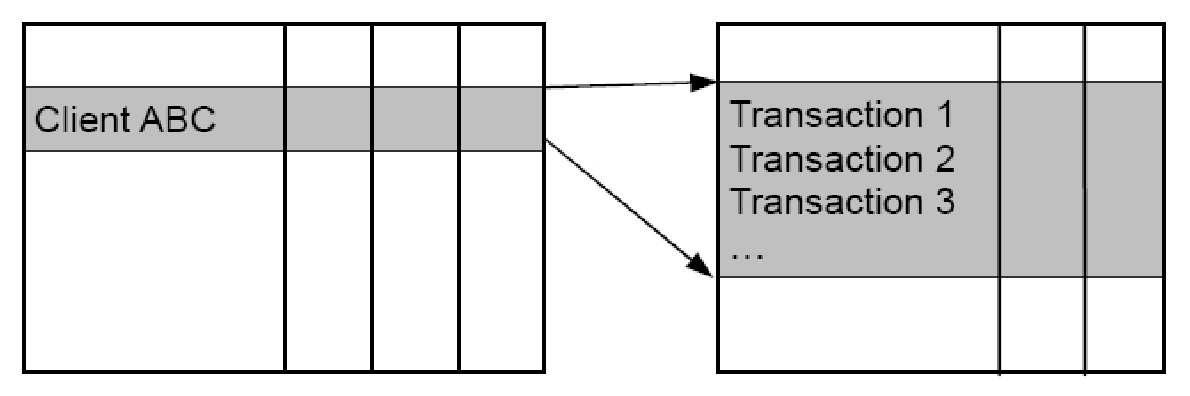
\includegraphics[width=8cm]{pics/master_detail.eps}
\end{center}
\caption{Master-detail tabulka}
\end{figure}

\paragraph{}
Pod�loha se v�dy spou�t� pro ty ��dky vedlej�� datov� matice, kter�
jsou v relaci s objektem z hlavn� datov� matice. Jako p��klad
uvedeme pod�lohu, kter� b�� na tabulce transakc�. V�dy se spust�
pouze pro ��dky transakc� pat��c� ur�it�mu klientovi. Nad t�mi prob�hne
verifikace n�jak� (po�ad� generov�n� se bude odv�jet od zp�sobu implementace)
relevantn� ot�zky generovan� pod�lohou a jako v�sledek pod�loha vyd� obecn�
re�ln� ��slo znamenaj�c� validitu dan� hypot�zy na zkouman� podmno�in�
��dk� vedlej�� datov� matice.
\paragraph{}
To znamen�, �e pro ka�d� objekt z hlavn� datov� matice pod�loha zkoumaj�c�
vedlej�� datovou matici vr�t� pr�v� jedno re�ln� ��slo. Takto vznikl�
sloupec se pro nad�lohu nebude nijak li�it od regul�rn�ho sloupce hlavn� datov� matice
a bude tedy zahrnut do generov�n� relevantn�ch ot�zek a pota�mo i hypot�z v nad�loze.
\subsection{Diskuze nad implementaci}
Z v��e popsan�ho je jasn�, �e implementace mus� vy�e�it n�kolik probl�mu.
Jejich �e�en� bylo podrobn� diskutov�no s vedouc�m diplomov� pr�ce Doc. RNDr. Janem Rauchem, CSc.
p�ibli�n� v n�sleduj�c�ch bodech.
\paragraph{}
Pro za��tek si je�t� jednou p�ipomeneme z�kladn� algoritmus generov�n�
relevantn�ch ot�zek a ov��ov�n� hypot�z pro dataminingovou proceduru 4ft miner.
%\clearpage
\begin{verbatim}
foreach(BitString condition in Conditions)
{
    foreach(BitString antecedent in Antecedents)
    {
        foreach(BitString succedent in Succedents)
        {
            ContingencyTable table = 
                ComputeTable(succedent, antecedent, condition);
            if (VerifyQuantifiers(table))
                result.Add(succedent, antecedent, condition);
        }
    }
}

\end{verbatim}

\subsubsection{Zp�sob b�hu pod�lohy}
\label{subtaskimplementation}
B�hem diskuze se vykrystalizovaly n�sleduj�c� t�i p��stupy, jak m��e pod�loha b�et.
\begin{description}
\item[P�edb�n� generov�n�]
Pod�loha by se spou�t�la p�edem na vedlej�� datov� matici. V�sledky ve form�
bu� virtu�ln�ch sloupc� a(nebo) bitov�ch �et�zk� by se p�echodn� skladovaly
v pam�ti �i ve form� serializovan�ch objekt� a p�i n�sledn�m b�hu nad�lohy
by se t�to p�edlo�ily. Podobn�m zp�sobem jsou implementov�ny nap��klad
st�vaj�c� nevirtu�ln� atributy -- ''Each value one category'', ''Ekvidistan�n� intervaly''
a ''Ekvifrekven�n� intervaly''.
\paragraph{}
V�hodou takov�ho p��stupu by byla mo�nost vyu��t st�vaj�c� v�hody implementace
metody GUHA v prost�ed� Ferda DataMiner a to zejm�na cache bitov�ch �et�zk�.
D�le by se mohly bez v�t��ch zm�n pou��t dataminingov� procedury jako pod�lohy,
v podstat� by se jednalo o jejich spu�t�n� na podmno�in� datov� matice m�sto
na cel� mno�in� ��dk�. Tak� takto implementovan� virtu�ln� atribut by �el
zapoj�t do zad�n� pro v�echny dosud implementovan� GUHA dataminingov�
procedury v prost�ed� Ferda DataMiner.
\paragraph{}
Hlavn�m d�vodem naps�n� p�edchoz�ho odstavce v podmi�ovac�m zp�sobu
se stala nemo�nost �k�lovatelnosti takov�ho �e�en�. U� i pro existuj�c�
vzorov� data virtu�ln� banky Barbora mohl nastat probl�m se zab�ranou
pam�ti pro vygenerovan� bitov� �et�zky. Po�et relevantn�ch ot�zek v zadan�
dataminingov� �loze v ��du tis�c� �i desetitis�c� je b�nou z�le�itost�.
Proto�e ka�d� relevantn� ot�zka v pod�loze znamen� nov� virtu�ln� sloupec
v hlavn� tabulce, nad kterou b�� hlavn� dataminingov� �loha, p�i �vaze
o velikosti po�adovan� opera�n� pam�ti (proto�e bitov� �et�zky krabi�ky
atribut� ve Ferda DataMiner uchov�vaj� pr�v� tam) se mus� po�et sloupc�
vyn�sobit po�tem ��dku hlavn� datov� matice.
\paragraph{}
P�i �vaze s matici banky Barbora o velikosti ��dov� kolem 5000 ��dku
a po�tem relevantn�ch ot�zek v pod�loze kolem 10000 n�m vznik� je�t� vcelku
p�ijateln� velikost zab�ran� RAM, nicm�n� je t�eba si uv�domit, �e velikost
zkouman� datov� tabulky pro �lohy bl��c� se re�ln� situaci je sp�e v ��dech
statis�c� a� mili�n� z�znam�. Toto je z�sadn� omezen� pro budouc� aplikace
prost�ed� Ferda DataMiner a takto navr�en� zp�sob implementace by omezil nejen
rela�n� roz���en� procedur implementovan�ch v r�mci dan� diplomov� pr�ce,
ale i p��pad\-n�ch dal��ch implementac� rela�n�ch roz���en� v budoucnu.
\paragraph{}
Z v��e uveden�ch d�vod� bylo tedy od tohoto zp�sobu implementace upu�t�no.
\item[�ekaj�c� vl�kna]Po zavr�en� p�edchoz�ho p��stupu bylo jasn�, �e �e�en�
p�edgenerovat si bitov� �et�zky do pam�ti nep�ipad� v �vahu. Za�al se hledat
zp�sob, jak virtu�ln� sloupce a tedy i bitov� �et�zky, generovat pr�b�n�,
v�dy na pokyn nad�lohy.
\paragraph{}
Vznikla n�sleduj�c� �vaha: proto�e nad�loha pot�ebovala ke zpracov�n� cel�
sloupec hlavn� datov� matice najednou, pod�loha by mohla b�et
jako dataminingov� procedura v samostatn�m vl�kn�, kter� by jako vstup m�la
pr�v� jednu podmno�inu ��dk� vedlej�� datov� matice pro jeden objekt z hlavn�
datov� matice. Tedy pro ka�d� objekt z hlavn� datov� matice by b�elo
jedno vl�kno pod�lohy, kter� by postupn� vracelo re�ln� ��sla, kter� by se formovala
do virtu�ln�ch sloupc�.
\paragraph{}
Skoro na prvn� pohled je v�ak jasn�, �e by muselo b�t spu�t�n stejn� po�et vl�ken
jako po�et ��dk� v hlavn� datov� matici. Idea nutnosti ��dov� tis�ce vl�ken pro v�po�et
by� jednoduch� �lohy (i nad tabulkou virtu�ln� banky Barbory) se autorovi dan�
diplomov� pr�ce zd�la jako velmi �patn� navr�ena z d�vod� p��li� velk�
re�ie opera�n�ho syst�mu na p�ep�nan� takov�ho po�tu vl�ken. Z dosavadn�ch
zku�enost� je vid�t, �e na b�n� dostupn�m osobn�m po��ta�i ��dov� i stovka vl�ken
v�t�inou p�edstavuje velk� vyt�en� komponent syst�mu.
\paragraph{}
Z v��e uveden�ch d�vod� bylo tedy od tohoto zp�sobu implementace upu�t�no.
\item[Generov�n� po kroc�ch]
P�edchoz� �vaha v�ak inspirovala autora pr�ce k jin�mu p��stupu k �e�en�. Jak je vid�t
z algoritmu generov�n� relevantn�ch ot�zek, kter� je uveden na po��tku t�to sekce,
dataminingov� �loha (v tomto p��pad� nad�loha) pot�ebuje v jednotliv�ch kroc�ch sv�ch cykl� pouze
\emph{jeden bitov� �et�zek}. Z tohoto vznikla idea navrhnout dataminingovou proceduru pro pod�lohu tak, aby um�la
poskytnout na po��d�n� ne n�jak� konkr�tn� sloupec nebo bitov� �et�zek, n�br� \emph{dal��} sloupec
a \emph{dal��} bitov� �et�zek anebo nic v p��pad� vy�erp�n� mo�n�ch sloupc�.
\paragraph{}
Z�sadn� rozd�l oproti dosud existuj�c�m (nevirtu�ln�m) atribut�m byl ten, �e tyto m�ly
celou mno�inu sv�ch bitov�ch �et�zk� v okam�iku p�ed za��tkem generov�n� zn�mou. Bitov�
�et�zky jsou v t�chto atributech identifikovateln� dle kl��e sklad�j�ciho se z id atributu a n�zvu
kategorie. Je zn�m celkov� po�et bitov�ch �et�zk�, tud� lze stanovit po�et celkov� vygenerovan�ch
relevantn�ch ot�zek. Je mo�n� p�istoupit k jak�mukoliv bitov�mu �et�zku na z�klad� kl��e.
\paragraph{}
Oproti tomu navrhovan� zp�sob implementace hypot�zov�ho atributu zaru�oval pouze to,
�e takov� atribut v okam�iku zavol�n� p��slu�n� metody bu� vyd� dal�� bitov� �et�zek
nebo ozn�m�, �e bitov� �et�zky u� vyd�vat nebude. Nen� tedy zn�m� a snadno p��stupn�
cel� mno�ina bitov�ch �et�zku p�ed za��tkem generov�n� (nad�lohou) relevantn�ch ot�zek.
Tud� nelze spo��tat ani p�edpokl�dan� po�et vygenerovan�ch relevantn�ch ot�tek,
proto�e hypot�zov� atribut jednodu�e reaguje bu� t�m, �e d� dal�� bitov� �et�zek
nebo ozn�m�, �e �et�zky do�ly.
\paragraph{}
V�hody tohoto �e�en� ve smyslu �k�lovatelnosti jsou z�ejm�. Pod�loha b�� synchronn�
s nad�lohou a v pam�ti se uchov�v� a p�ed�v� pouze jeden bitov� �et�zek v jednom okam�iku.
Pot�, co nad�loha p�ejde na dal�� krok generov�n� a po��d� virtu�ln� atribut o dal�� bitov� �et�zek,
tento zavol� svoji metodu MoveNext a vyd� dal�� �et�zek. P�edchoz� vygenerovan� �et�zky
se nikde neukl�daj� a nezab�raj� pam�.
\paragraph{}
Nev�hody tohoto �e�en� jsou ji� nazna�eny
v��e a budou podrobn�ji probr�ny d�le. Po diskuzi s vedouc�m diplomov� pr�ce se autor rozhodl
implementovat rela�n� roz���en� dataminingov�ch procedur pr�v� t�mto zp�sobem,
proto�e p��padn� nev�hody a jin� p��stup k �e�en� znamenaly sp�e nepohodl� pro program�tora, av�ak
nijak nenaru�ovaly princip metody GUHA jako takov�. Nav�c poskytovaly z�kladn� v�hodu
�k�lovatelnosti -- z principu n�vrhu lze zaru�it, �e �loha skon�� i na velk�ch tabulk�ch,
nevy�erp� RAM nebo po�et povolen�ch b��c�ch vl�ken v syst�mu. M��e se st�t, �e
pob�� del�� dobu, ale skon�� korektn�.
\end{description}
\subsection{D�sledky zvolen�ho zp�sobu}
Zde budou pops�ny d�sledky, kter� m�lo zvolen� �e�en� implementaci a spolupr�ci
s ji� existuj�c�mi moduly metody GUHA v prost�ed� Ferda DataMiner.
\subsubsection{Vypnut� cache bitov�ch �et�zku}
Nejpodstatn�j��m d�sledkem byla nemo�nost pou��vat st�vaj�c� cache bitov�ch
�et�zk�. Ta tot� funguje tak, �e uchov�v� bitov� �et�zky pro atributy
(pro v�echny atributy je spole�n�) a v p��pad� pot�eby vy�azuje z cache
m�lo pou��van� bitov� �et�zky na z�klad� n�jak� strategie. V p��pad�,
�e v cache pot�ebn� bitov� �et�zek neexistuje, po��d� o n�j p��mo
pot�ebn� atribut na z�klad� jednozna�n�ho identifik�toru.
\paragraph{}
Jak u� bylo zm�n�no v��e, takov� p��stup by se zvolen�m zp�sobem implementace
nefungoval -- p�edpokl�d� toti� mo�nost p��stupu ke v�em bitov�m �et�zk�m
atributu. N�vrh hypot�zov�ho virtu�ln�ho atributu s t�mto nepo��t� -- um�
d�t pouze ''dal��'' bitov� �et�zek bez mo�nosti zjistit, kter� dal�� to bude, jak�
bude m�t identifik�tor, ke kter� kategorii bude pat�it atd. Z t�chto d�vod�
ne�lo st�vaj�c� cache pro hypot�zov� virtu�ln� atribut pou��t. Pou�it�
cache bitov�ch �et�zk� u ostatn�ch bu� existuj�c�ch nebo nov� implementovan�ch
krabi�ek atribut� z�stalo beze zm�ny, proto�e se pro tyto krabi�ky nic nezm�nilo.
\subsubsection{Rozd�len� na krabi�ky}
Dal�� �vahou bylo, zda implementovat hypot�zov� virtu�ln� atribut
jako dv� krabi�ky nebo jednu spole�nou. St�vaj�c� nevirtu�ln�
atributy se v p��pad� pot�eby generov�n� boolsk�ch atribut� zapojuj� do krabi�ky
''AtomSetting''. Ta zajist� generov�n� koeficient� pro booleovsk� atribut.
\paragraph{}
V p��pad� hypot�zov�ho virtu�ln�ho atributu by ne�la pou��t st�vaj�c� krabi�ka
pro generov�n� koeficient� ''AtomSetting'', proto�e pracuje s po�adavkem ''poskytni
p�esn� tento bitov� �et�zek'', kde�to hypot�zov� atribut by um�l zpracovat pouze
po�adavek ''poskytni dal�� bitov� �et�zek''. Tud� krabi�ka pro generov�n� koeficient�
vyu�iteln� pouze pro hypot�zov� virtu�ln� atribut by se se musela tak� naprogramovat.
\paragraph{}
Po �vaze se autor rozhodl neimplementovat zvl�tn� krabi�ku pro generov�n�
koeficient� pro hypot�zov� virtu�ln� atribut z n�sleduj�c�ch d�vod�.
\begin{description}
\item[Pot�eba pouze jednoho koeficientu] Po diskuzi s vedouc�m pr�ce
bylo rozhodnuto, �e p�i generov�n� koeficient� pro booleovsk� atribut
bude pot�eba implementovat pouze podmno�iny d�lky jedna -- viz \ref{coefficients}.
Krabi�ka ''AtomSetting'' pro hypot�zov� virtu�ln� atribut by byla nadbyte�n�,
proto�e by tam chyb�lo u�ivatelsk� nastaven�, v�e se odehr�valo ''pod kapotou''.
Nebyl tedy d�vod tuto krabi�ku vytv��et.
\item[Nadbyte�n� komunikace krabi�ek p�es ICE] Nav�c by tato krabi�ka, kter�
by se napojila za hypot�zov� virtu�ln� atribut, znamenala komunikaci p�es ICE.
Proto�e idea implementace spo��v� v synchronn�m b�hu nad- a pod�lohy, kde
nad�loha uvnit� sv�ch cykl� (nap��klad pro sukcedent) vol� pod�lohu, kter� j�
p�ed�v� bistringy, je pot�eba zajistit toto p�ed�v�n� plynule, aby
se hlavn� �loha p��li� nezpomalovala �ek�n�m na bitov� �et�zek od pod�lohy.
\paragraph{}
 Proto�e
ze zku�enost� z�skan�ch p�i programov�n� prost�ed� Ferda DataMiner je�t�
jako studentsk�ho projektu autor v�d�l, �e komunikace krabi�ek p�es
rozhran� ICE je relativn� pomal� (s ohledem na skute�nost, �e na komunikaci
p�es ICE by bylo t�eba �ekat p�i ka�d�m kroku  \verb+foreach+ cyklu),
bylo rozhodnuto zajistit generov�n� atributu
a koeficientu v jedn� krabi�ce a t�m zrychlit b�h hypot�zov�ho
virtu�ln�ho atributu.
\end{description}
\subsubsection{Buffer bitov�ch �et�zk�}
P�i lad�n� prvotn� implementace hypot�zov�ho virtu�ln�ho atributu
se zjistilo, �e a�koliv zvolen� n�vrh zaru�� �k�lovatelnost
a jistotu toho, �e �loha by� za del�� dobu dob�hne a nezabere
zbyte�nou pam�, doba b�hu celkov� �lohy je ne�m�rn� dlouh�.
\paragraph{}
D�vod dlouh�ho b�hu �lohy s virtu�ln�m atributem celkem logicky spo��val
v neexistenci jak�hokoliv cacheov�n� bitov�ch �et�zk� poskytovan�ch
virtu�ln�m hypot�zov�m atributem. P�i prvotn�m n�vrhu autor a vedouc�
diplomov� pr�ce na tento fakt nebrali p��li� ohled, proto�e sp�e diskutovali
o dlouho\-dob�j��ch dopadech zvolen�ho zp�sobu implementace. Velk� rozd�l v rychlostech b�hu
�lohy byl je�t� umocn�n faktem, �e v�echny dosavadn� GUHA procedury byly implementov�ny
s pou�it�m cache bitov�ch �et�zk� a generov�n� bitov�ch �et�zk� p�i b�hu �lohy prob�hlo
pouze poprv� a pot� se na��taly z cache. Proto hypot�zov� atribut, kter� ��dnou cache
nepou��val, zp�soboval opravdu velk� zpomalen� b�hu �lohy, byl-li do ni zapojen.
\paragraph{}
Pod�v�me-li se na algoritmus 4ft mineru uveden�ho v��e a p�edstav�me-li si ho
jako nad�lohu, do kter� bude zapojen minim�ln� jeden virtu�ln� hypot�zov� atribut
(nap��klad jako sukcedent), tak bude jasn�, �e tento algoritmus pob�� opravdu pomalu.
Zapojen� virtu�ln�ho atributu do sukcedentu je pro tento miner ''nejhor�� p��pad'',
proto�e bitstringy jim generovan� jsou pou��vany ve vnit�n�m \verb+foreach+ cyklu,
a v p��pad� nepou��van� cache to znamen�, �e uvnit� tohoto cyklu se \emph{poka�d�} spust�
pod�loha (vnit�n� miner), aby mohla nad�loze poskytnout bitstring.
\paragraph{}
P�i v�� snaze autora dan� pr�ce jakkoliv urychlit b�h �lohy se zapojen�m hypot�zov�m
atributem vych�zelo najevo, �e od p�vodn� pl�novan� implementace prost� jak�hokoliv
cacheov�n� bude nutn� upustit. P�i kr�tk�m otestov�n� a optimalizaci dosud naimplementovan�ho
k�du krabi�ky autor byl schopen dos�hnout rozumn� doby b�hu �lohy (v ��du des�tek minut)
p�i omezen� maxim�ln�ho po�tu virtu�ln�ch sloupc� a pota�mo i bitov�ch �et�zk� vygenerovan�ch
krabi�kou virtu�ln�ho atributu na 15-20. P�i zv��en� maxim�ln�ho po�tu virtu�ln�ch sloupc�
na 50 doba b�hu jednoduch� �lohy se pohybovala v ��du hodin.
\paragraph{}
Proto�e b�n� po�ty vygenerovan�ch relevantn�ch ot�zek v procedur�ch GUHA se pohybuj� v ��dech
tis�c� a� desetitis�c� p�i pot�ebn� dob� b�hu sp�e v ��du minut, bylo z�ejm�, �e
zpomaluj�c�m faktorem byla pr�v� absence cacheov�n� bitov�ch �et�zk� pro virtu�ln� atribut.
Bylo tedy rozhodnuto upustit od kanonick�ho implementa�n�ho �e�en� a autor naimplementoval
cache i pro virtu�ln� atributy.
\section{Atributy}
Zde bude pops�na podstata �lohy, kterou bylo nutn�
vy�e�it pro implementaci atribut� v prost�ed�
Ferda DataMiner. Podrobn�j�� popis princip� fungov�n� dan�ch
atribut� je uveden v dan� diplomov� pr�ci v sekci \ref{cileatributy}.
\subsection{Ekvidistan�n� intervaly}
V r�mci implementace funk�nosti tohoto atributu byly vyu�ity algoritmy
pro vytvo�en� ekvidistan�n�ch interval� p�ipraven� T.Kucha�em
v r�mci jeho diplomov� pr�ce uveden� jako \cite{kuchar}. Tyto algoritmy
byly adaptov�ny z prost�ed� projektu Rel-Miner T.Karbana a p�ipraveny
pro vyu�it� v prost�ed� Ferda DataMiner. Autor dan� diplomov� pr�ce
vytvo�il pro dan� atribut krabi�ku v prost�ed� Ferda DataMiner,
jej� funk�nost bude detailn� pops�na v kapitole \ref{implementationdetails}.

\subsection{Ekvifrekven�n� intervaly}
V r�mci implementace funk�nosti tohoto atributu byly vyu�ity algoritmy
pro vytvo�en� ekvifrekven�n�ch interval� p�ipraven� T.Kucha�em
v r�mci jeho diplomov� pr�ce uveden� jako \cite{kuchar}. Tyto algoritmy
byly adaptov�ny z prost�ed� projektu Rel-Miner T.Karbana a p�ipraveny
pro vyu�it� v prost�ed� Ferda DataMiner. Autor dan� diplomov� pr�ce
vytvo�il pro dan� atribut krabi�ku v prost�ed� Ferda DataMiner,
jej� funk�nost bude detailn� pops�na v kapitole \ref{implementationdetails}.
\subsection{Statick� atribut}
V r�mci implementace funk�nosti tohoto atributu byla vytvo�ena krabi�ka,
kter� umo��ovala spou�t�n� modulu pro ru�n� �pravu atributu. Atribut
(p�esn�ji kategorie v atributu) mohly b�t p�edem vytvo�eny nap��klad
v��e uveden�mi krabi�kami ekvidistan�n�ch nebo ekvifrekven�n�ch interval�.
\subsection{Modul pro �pravu atributu}
Tento modul je spou�t�n nad krabi�kou ''Statick� atribut'' a umo��uje
ru�n� �pravu kategori� v atributu. P�i n� u�ivatel m��e jak upravovat
ji� p�edp�ipraven� kategorie, tak i vytv��et kategorie nov�. Upravovan�
atribut m��e b�t i zcela pr�zdn� a kategorie mohou b�t vytvo�eny
u�ivatelem kompletn� od za��tku.
\paragraph{}
Modul zaru�uje korektnost ru�n� p�idan�ch kategori� (zaru�� nap��klad
disjunktnost interval�, jak je po�adov�no p�i tvorb� �lohy pro dataminingovou
proceduru). Vyu��v� algoritm� ji� implementovan�ch v r�mci diplomov� pr�ce
T.Kucha�e uveden� jako \cite{kuchar}. Funk�nost tohoto modulu bude detailn� pops�na
v kapitole \ref{implementationdetails}.
\chapter{Implementace}
V t�to kapitole budou uvedeny a pops�ny implementovan�
procedury a krabi�ky v�etn� uveden� n�kter�ch nejd�le�it�j��ch
detail� implementace.

\label{implementationdetails}
\section{Agrega�n� atribut}
Podrobn�j�� popis ��elu virtu�ln�ho agrega�n�ho atributu
byl uveden v p�ed\-choz�ch kapitol�ch. Zde podrobn� probereme
naimplementovanou funk�nost v�etn� popisu vytvo�en� krabi�ky.
\subsection{Detaily implementace}
Agrega�n� virtu�ln� atribut poskytuje mo�nost spojit dv�
datov� matice (datab�zov� tabulky) na z�klad� zadan�ho kl��e
a volby v�sledn�ho sloupce z vedlej�� datov� matice.
V�sledn� sloupec lze zapojit do dataminingov� �lohy GUHA stejn� jako
v�sledn� sloupec, kter� poskytuje krabi�ka ''Sloupec''.
\paragraph{}
D�le dan� atribut m��e v budoucnu vyu��vat mo�nosti pr�ce s SQL funkcemi
d�ky pou�it� stejn�ho postupu jako p�i nadefinov�n� odvozen�ho sloupce.
Tato funk�nost v�ak nebyla implementov�na z d�vodu pracnosti, ale
m��e b�t lehce dopln�na pozd�ji -- pravd�podobn� autorem dan� diplomov� pr�ce
mimo diplomovou pr�ci, ale v r�mci dal��ho roz���ov�n� prost�ed�
Ferda DataMiner.
\subsection{Krabi�ka}
Dan� krabi�ka reprezentuje v��e popsan� agrega�n�
virtu�ln� atribut z u�ivatelsk�ho hlediska.
\subsubsection{Seznam z�suvek}
\begin{description}
\item[Hlavn� datov� tabulka] 
Do t�to z�suvky se zapojuje krabi�ka reprezentuj�c� hlavn�
datovou matici.
\item[Vedlej�� datov� tabulka]
Do t�to z�suvky se zapojuje krabi�ka reprezentuj�c� vedlej��
datovou matici.
\end{description}
\subsubsection{Seznam vlastnost�}
\begin{description}
\item[S�mantika] 
Umo�n� vybrat s�mantiku sloupce. S�mantika v prost�ed� Ferda DataMiner
byla podrobn�ji pops�na v \ref{datasemantics}. U�ivatel m��e tedy vybrat
z mo�nost� \emph{Nomin�ln�, Ordin�ln�, Cyklick� ordin�ln�, Kardin�ln�}.
\item[Id sloupec hlavn� datov� tabulky] 
Zde se vybere sloupec ze seznamu na\-b�zen�ch sloupc� hlavn� datov� tabulky.
Z�znamy z dan�ho sloupce budou pou��ty jako kl��e pro z�znamy z hlavn� datov� tabulky
p�i spojen� hlavn� a vedlej�� datov� tabulky.
\item[Id sloupec vedlej�� datov� tabulky] 
Zde se vybere sloupec ze seznamu na\-b�zen�ch sloupc� hlavn� datov� tabulky.
Z�znamy z dan�ho sloupce budou pou��ty jako kl��e pro z�znamy z vedlej�� datov� tabulky
p�i spojen� hlavn� a vedlej�� datov� tabulky.
\end{description}
\subsubsection{Seznam vlastnost� pouze pro �ten�}
Vlastnosti pouze pro �ten� obecn� v prost�ed� Ferda DataMiner
slou�� k informov�n� u�ivatele o vlastnostech zkouman� krabi�ky.
\paragraph{}
Vlastnosti pouze pro �ten� pro danou krabi�ku jsou shodn� s vlastnostmi pro �ten�
krabi�ky ''Sloupec''.
\begin{description}
\item[Datov� typ] 
Zobraz� datov� typ hodnot z�znam� ve sloupci.
\item[Pr�m�r] 
Zobraz� pr�m�r hodnot z�znam� ve sloupci.
\item[Navz�jem r�zn� hodnoty] 
Zobraz� po�et z�znam� s navz�jem r�zn�mi hodnotami ve sloupci.
\item[Maximum] 
Zobraz� maxim�ln� hodnotu ze v�ech hodnot z�znam� ve sloupci.
\item[Minimum] 
Zobraz� minim�ln� hodnotu ze v�ech hodnot z�znam� ve sloupci.
\item[Standardn� odchylka] 
Zobraz� hodnotu standardn� odchylky ze v�ech hodnot z�znam� ve sloupci.
\item[Variabilita] 
Zobraz� hodnotu variability ze v�ech hodnot z�znam� ve sloupci.
\end{description}

\section{Hypot�zov� atribut}
Podrob\-n�j�� po\-pis ��elu vir\-tu�l\-n�ho hypo\-t�\-zo\-v�ho atri\-bu\-tu
byl uve\-den v p�ed\-cho\-z�ch ka\-pi\-to\-l�ch. Zde ro\-ze\-be\-reme
na\-implemen\-tovanou funk�\-nost v�et\-n� po\-pi\-su vyt\-vo\-�en�ch kra\-bi�ek.
\subsection{Detaily implementace}
Hypo\-t�zov� vir\-tu�ln� atribut ge\-ne\-ruje vir\-tu�ln� sloupce (p�esn�ji p��mo 
bi\-tov� �et�zky) na z�k\-lad� zad�n� pod\-�lohy. Tato se za\-d�v� ob\-dobn� jako
b�n� data\-mining\-ov� �loha pro ji� existuj�c� pro\-ce\-dury. Roz\-d�lem
je p�e\-dev��m pos\-kytovan� v�s\-ledek. Hypo\-t�zov� virtu�ln� atri\-but
ne\-poskytuje v�s\-ledek pro pro\-hl�en� u�i\-vatelem (na\-rozd�l od b�\-n�ch
nerela�n�ch procedur), ale pro ne\-rela�n� data\-miningovou pro\-ceduru,
do zad�n� kter� je zahrnut jako booleovsk� atribut.
\paragraph{}
Jako sou��st implementace hypo\-t�zov�ho virtu�ln�ho atri\-butu v pro\-st�ed�
Ferda DataMiner byly vyt\-vo�eny kra\-bi�ky pro 4ft vir\-tu�ln� hypo\-t�zov� atri\-but a 
SD4ft virtu�ln� hypo\-t�zov� atribut. Rovn� byly pro\-ve\-deny �pravy n�k\-ter�ch modul�,
kter� pou��vaj� krabi�ky data\-minigov�ch pro\-cedur.
\paragraph{}
Jak u� bylo zm�n�no v \ref{subtaskimplementation}, kra\-bi�ky 4ft a SD4ft
virtu�l\-n�ho atributu gene\-ruj� rov\-nou bitov� �et�zky pro druh koeficientu
''jedno\-prvkov� pod\-mno�ina''. V prost�ed� Ferda Data\-Miner pro\-to vystupuj� na m�st�
kra\-bi�ky jak ''AtomSetting'', tak krabi�ky atri\-butu.
\subsubsection{Generov�n� kolekce}
P�i implementov�n� dle n�vrhu z \ref{subtaskimplementation} se autor rozhodl vyu��t
nov�ch vlastnost�, kter� nab�zel jazyk C\# ve verzi 2.0 a to konkr�tn� zaveden�
kl��ov�ho slova \verb+yield+ pro velmi snadn� implementov�n�
iter�toru (v�ce viz na\-p��\-klad na \verb+http://msdn2.microsoft.com/en-us/library/9k7k7cf0.aspx+).
\paragraph{}
Tato vlastnost nov�ho C\# usnadnila implementov�n� p��stupu ''poskytni dal�� bitov� �et�zek'',
proto�e velmi zjednodu�en� �e�eno umo��uje vr�tit kolekci prvk�, kterou lze proch�zet
pomoc� cyklu foreach, ani� by byly dop�edu zn�m� prvky v dan� kolekci. Ta se
tot� generuje dynamicky, co� se n�m hod� pr�v� p�i implementaci kolekce bitov�ch �et�zk�,
kter� jsou zisk�vany metodou ''poskytni dal�� bitov� �et�zek''.

\subsubsection{Count vector}
Pro generov�n� bitov�ho �et�zku spr�vn� d�lky (tzn. stejn� d�lky jako bitov�
�et�zky v nad�loze) je nutn� v�d�t, kolik ��dk� z vedlej�� datov� matice se v�e
ke ka�d�mu objektu z hlavn� datov� matice. Potom bude mo�n� generovat virtu�ln� sloupec
spr�vn� d�lky -- viz \ref{subtaskimplementation}.
\paragraph{}
Tato informace je z�sk�v�na pomoc� tzv. \emph{CountVectoru}, kter� na $i$-t� pozici
obsahuje po�et ��dk� vedlej�� datov� matice pat�ic�ch $i$-t�mu objektu z hlavn�
datov� matice (to samoz�ejm� p�edpokl�d� set��d�n� obou matic dle stejn�ho kl��e).
\paragraph{}
Za pou�it� \emph{CountVectoru} lze generovat cel� virtu�ln� sloupec, pota�mo odpov�daj�c�
bitov� �et�zek, ji� pom�rn� snadno. Pod�loha gene\-ruj�c� vir\-tu�ln� sloup\-ce
jako v�sledek platnosti rele\-vantn�ch ot�zek, bude po��tat na pod\-mno�in� ��dk� zji�t�n�
z informace dan� \emph{CountVectorem}. P�ed spu�t�n�m gene\-rov�n� rele\-vantn�ch ot�zek se pro
ka�d� objekt z hlavn� datov� matice vytvo�� tzv. \emph{masky}, co� jsou bi\-tov� �et�zce s d�l\-kou rov\-naj�c� se po�tu z�znam� ve vedlej\-�� da\-tov� matici a jejich po�et odpo\-v�d� po�tu ob\-jekt� v hlav\-n� datov� matici. Ka�d�
objekt z hlavn� datov� matice m� vytvo�enou svoji masku. Bitov� �et�zek masky pro $i$-t� ��dek
hlavn� datov� matice obsahuje jedni�ky na pozic�ch odpov�daj�c�ch um�st�n� z�znam� z vedlej��
datov� matice vztahuj�c�ch se k $i$-t�mu ��dku hlavn� datov� matice. Nap��klad, m�me-li v tabulce klient� dva klienty
a v tabulce transakc� 10 transakc�, 4 pro prvn�ho klienta a 6 pro druh�ho, pak vzniknou dv� masky
o d�lce 10 bit�. Maska pro prvn�ho klienta bude obsahovat jedni�ky na pozic�ch 0-3 a jinak nuly
a maska pro druh�ho klienta bude obsahovat jedni�ky na pozic�ch 4-9 a jinak nuly.
\paragraph{}
Takto vygenerovan� masky se aplikuj� na bitov� �et�zky gene\-ro\-van� at\-ri\-bu\-ty v zad�n� pod\-�lohy ope\-rac� AND,
��m� se vynuluj� hodnoty na pozic�ch bitov�ho �et�zku, kter� neodpov�daj� pr�v� zkouman�mu ob\-jektu z hlav\-n� ma\-tice. Pod\-�loha tedy v�dyc\-ky pro\-b�hne pouze pro po\-�adovan� ��d\-ky ved\-lej�� datov� ma\-tice, jak je po�a\-dov�no.

\subsubsection{Cache bitov�ch �et�zk�}
Z d�vod� zm�n�n�ch v \ref{subtaskimplementation} byla naimplementov�na jin� cache
pro bi\-tov� �et�zky generovan� hypot�zov�mi atributy. Dle principu fungov�n�
je to sp�e buffer ne� cache -- uchov� prvn�ch N bi\-tov�ch �et�zk� vy\-gene\-rovan�ch
hypo\-t�zov�m atributem, kter� mohou b�t pot� pou�ity pro b�h nad�lohy. Velikost N
byla stanovena konstantn�, proto�e, jak bylo zji�t�no p�i hlub��m zkoum�n� zp�sobu implementace
st�vaj�c�ch procedur p�i programov�n� hypot�zov�ch atribut�,
ani p�vodn� cache pro bitov� �et�zky neobsahuje ��dnou logiku pro stanoven� sv� velikosti.
\subsubsection{�prava existuj�c�ch dataminingov�ch procedur}
Existuj�c� data\-miningov� proce\-dury muse\-ly b�t roz\-���eny o me\-to\-dy umo�\-�uj�\-c�
gene\-rov�n� a ve\-rifi\-kaci rele\-vantn�ch ot�zek, bez ge\-ne\-rov�n� hy\-pot�z a s imple\-mentaci
v��e zm�n�n�ho enumer�toru. Rovn� bylo nut\-n� roz\-���it data\-miningov� pro\-cedury
o mo�\-nost pr�ce s jin�m druhem cache pro bi\-tov� �e\-t�zky.
\subsubsection{P��nos pro budouc� implementace}
V��e uveden� postupy jsou navr�eny a implementov�ny co nejobecn�ji. Auto\-r�m imple\-mentace
rela�n�ch roz���en� dal��ch datamingov�ch procedur se t�mto m��e jejich pr�ce velmi usnadnit.
Mohou pou��vat cache pro bitov� �et�zky virtu�ln�ch atribut�, CountVector, masky a dal��
navr�en� postupy.

\subsection{Krabi�ky}
\subsubsection{Krabi�ka 4ft virtu�ln� booleovsk� atribut}
Dan� krabi�ka reprezentuje v��e popsan� hypot�zov�
virtu�ln� atribut z u�ivatelsk�ho hlediska. V sou�asn� dob� lze do zad�n�
�lohy zapojit pouze jednou krabi�ku hypot�zov�ho atributu.
\subsubsection{Seznam z�suvek}
Z�suvky jsou shodn� s krabi�kou ''4ft-Miner'' a� na v�jimky, jejich� popis n�sleduje.
\begin{description}
\item[Hlavn� datov� tabulka] 
Do t�to z�suvky se zapojuje krabi�ka reprezentuj�c� hlavn�
datovou matici.
\end{description}
\subsubsection{Seznam vlastnost�}
Vlastnosti jsou shodn� s krabi�kou ''4ft-Miner'' a� na v�jimky, jejich� popis n�sleduje.
\begin{description}
\item[Maxim�ln� po�et relevantn�ch ot�zek]
Zde se zad�v� maxim�ln� po�et relevantn�ch ot�zek, kter� m��e virtu�ln� atribut vygenerovat.
\end{description}
Pro �sp�n� spu�t�n� �lohy, do n� je zapojena tato rela�n� procedura, je nutn�
zvolit kl��, podle kter�ho se budou identifikovat z�znamy ve vedlej�� datov� matici
oproti z�znam�m v hlavn� datov� matici. Pro hlavn� datovou matici, kter� je zapojena
do z�suvky se stejn�m jm�nem, se zvol� jej� prim�rn� kl�� pomoc� vlast\-nost� krabi�ky
''Tabulka'' se jm�nem ''Sloupce prim�rn�ho kl��e''. Pro vedlej�� datovou matici,
ze kter� se vytv��ej� atributy pro zapojen� do krabi�ky rela�n� procedury, se zvol�
slou\-pec ob\-sahu\-j�c� z�z\-namy ji� vyb\-ra\-n�ho v p�ed\-choz�m kroku kl��e z hlavn� datov� matice.
\paragraph{}
�loha po��t� s integritou dat: existuje-li ve vedlej�� datov� matici z�znam, kter�mu
neodpov�d� ��dn� z�znam hlavn� datov� matice, �loha skon�i chybou. V�z\-nam m��eme ch�pat
n�sleduj�c�m zp�sobem: m�me-li data\-b�zi banky a v n� tabul\-ky pro klienty a transakce
identifikovan� nap��klad dle id klienta, lze po��tat s t�m, �e pro ka�dou transakci bude
existovat klient, kter� ji provedl. P��pad existence klienta, kter� ��dn� transakce neprovedl,
m��e b�t naopak b�n� a p�i takov� situaci �loha prob�hne korektn�.

\subsubsection{Krabi�ka SD4ft virtu�ln� booleovsk� atribut}
Dan� krabi�ka reprezentuje v��e popsan� hypot�zov�
virtu�ln� atribut z u�ivatelsk�ho hlediska.
\subsubsection{Seznam z�suvek}
Z�suvky jsou shodn� s krabi�kou ''SD4ft-Miner'' a� na v�jimky, jejich� popis n�sleduje.
\begin{description}
\item[Hlavn� datov� tabulka] 
Do t�to z�suvky se zapojuje krabi�ka reprezentuj�c� hlavn�
datovou matici.
\end{description}
\subsubsection{Seznam vlastnost�}
Vlastnosti jsou shodn� s krabi�kou ''SD4ft-Miner'' a� na v�jimky, jejich� popis n�sleduje.
\begin{description}
\item[Maxim�ln� po�et relevantn�ch ot�zek]
Zde se zad�v� maxim�ln� po�et relevantn�ch ot�zek, kter� m��e virtu�ln� atribut vygenerovat.
\end{description}
Pro �sp�n� spu�t�n� �lohy je po�adov�no spr�vn� volba kl��� hlavn� a vedlej�� datov� matice
stejn� jako v p��pad� 4FT virtu�ln�ho boolovsk�ho atributu - viz v��e.

\section{Ekvidistan�n� intervaly}
Z d�vod� popsan�ch v \ref{zmenazadani} byla imple\-men\-tov�na kra\-bi�\-ka atri\-butu
pro ge\-ne\-rov�n� ekvi\-dis\-tan�\-n�ch inter\-val�.
\subsection{Detaily implementace}
Implementace krabi�ky vyu��v� algoritm�, kter� byly p�ipraveny T.Kucharem
v r�mci diplomov� pr�ce \cite{kuchar} a p�vodn� poch�zej� od T.Karbana -- viz
\cite{relminer}. Autor se proto soust�edil na implementov�n� samotn� krabi�ky.
\subsection{Krabi�ka}
\subsubsection{Seznam z�suvek}

\begin{description}
\item[Sloupec] 
Do t�to z�suvky se zapojuje krabi�ka reprezentuj�c� sloupec dat, nad kter�m budou
vytvo�eny ekvidistan�n� intervaly.
\end{description}
\subsubsection{Seznam vlastnost�}
\begin{description}
\item[Po�et kategori�]
Zde se zad�v� po�et interval�, kter� m� atribut vy\-ge\-ne\-ro\-vat.
\item[X kategorie]
Zde se zad�v� kategorie chyb�j�c� informace.
\item[Dom�na]
Zde se zad�v� typ vybran� dom�ny sloup\-ce trans\-formov�n� do kate\-gori�. 
U�ivatel m��e vyb\-rat z mo�nosti ''Cel� aktu�ln� dom�na'' a ''U�ivatelem definov�na dom�na''.
Prvn� mo�\-nost nas\-tav� vyt\-v��en� kate\-gorie pro ka�dou hod\-notu z aktu�ln� do\-m�ny sloupce,
druh� mo�\-nost nas\-tav� omezen� pro pou�itou dom�nu na z�klad� hodnot vlastnost� ''Od'' a ''Do''.
\item[Od]
P�i zvolen� u�iva\-telem defi\-novan� dom�ny kate\-gorie budou vyt\-vo�eny pouze
pro hodnoty z aktu�ln� dom�ny sloupce, kter� jsou v�t\-�� nebo rovny hod\-not� dan� vlast\-nosti.
\item[Do]
P�i zvolen� u�ivatelem defi\-novan� dom�ny kate\-gorie budou vyt\-vo�eny pouze
pro hodnoty z aktu�ln� do\-m�ny sloupce, kter� jsou men\-�� nebo rovny hod\-not� dan� vlast\-nosti.
\item[N�zev ve v�sledc�ch] Atri\-but je uveden v hypo\-t�z�ch pod dan�m n�z\-vem.
\item[S�mantika] 
Umo�n� vybrat s�mantiku sloupce. S�mantika v prost�ed� Ferda DataMiner
byla podrobn�ji pops�na v \ref{datasemantics}. U�ivatel m��e tedy vybrat
z mo�nost� \emph{Nomin�ln�, Ordin�ln�, Cyklick� ordin�ln�, Kardin�ln�}.
\end{description}


\section{Ekvifrekven�n� intervaly}
Z d�vod� popsan�ch v \ref{zmenazadani} byla implemen\-tov�na krabi�ka atributu
pro ge\-ne\-ro\-v�n� ekvi\-frek\-ven�n�ch interval�.
\subsection{Detaily implementace}
Implementace krabi�ky vyu��v� algoritm�, kter� byly p�ip\-ra\-ve\-ny T.Ku\-cha\-�em
v r�mci dip\-lomov� pr�ce \cite{kuchar} a p�\-vod\-n� poch�zej� od T.Kar\-bana -- viz
\cite{relminer}. Autor se proto soust�edil na implementov�n� samotn� krabi�ky.
\subsection{Krabi�ka}
\subsubsection{Seznam z�suvek}

\begin{description}
\item[Sloupec] 
Do t�to z�suvky se zapojuje krabi�ka reprezentuj�c� sloupec dat, nad kter�m budou
vytvo�eny ekvifrekven�n� intervaly.
\end{description}
\subsubsection{Seznam vlastnost�}
\begin{description}
\item[Po�et kategori�]
Zde se zad�v� po�et interval�, kter� m� atribut vy\-ge\-ne\-ro\-vat.
\item[X kategorie]
Zde se zad�v� kategorie chyb�j�c� informace.
\item[Dom�na]
Zde se zad�v� typ vybran� dom�ny sloup\-ce trans\-formov�n� do kate\-gori�. 
U�ivatel m��e vyb\-rat z mo�nosti ''Cel� aktu�ln� dom�na'' a ''U�ivatelem definov�na dom�na''.
Prvn� mo�\-nost nas\-tav� vyt\-v��en� kate\-gorie pro ka�dou hod\-notu z aktu�ln� do\-m�ny sloupce,
druh� mo�\-nost nas\-tav� omezen� pro pou�itou dom�nu na z�klad� hodnot vlastnost� ''Od'' a ''Do''.
\item[Od]
P�i zvolen� u�iva\-telem defi\-novan� dom�ny kate\-gorie budou vyt\-vo�eny pouze
pro hodnoty z aktu�ln� dom�ny sloupce, kter� jsou v�t\-�� nebo rovny hod\-not� dan� vlast\-nosti.
\item[Do]
P�i zvolen� u�ivatelem defi\-novan� dom�ny kate\-gorie budou vyt\-vo�eny pouze
pro hodnoty z aktu�ln� do\-m�ny sloupce, kter� jsou men\-�� nebo rovny hod\-not� dan� vlast\-nosti.
\item[N�zev ve v�sledc�ch] Atri\-but je uveden v hypo\-t�z�ch pod dan�m n�z\-vem.
\item[S�mantika] 
Umo�n� vybrat s�mantiku sloupce. S�mantika v prost�ed� Ferda DataMiner
byla podrobn�ji pops�na v \ref{datasemantics}. U�ivatel m��e tedy vybrat
z mo�nost� \emph{Nomin�ln�, Ordin�ln�, Cyklick� ordin�ln�, Kardin�ln�}.
\end{description}

\section{Statick� atribut}
Z d�vod� popsan�ch v \ref{zmenazadani} byla implementov�na krabi�ka
statick�ho atributu, kter� umo�n� ru�n� �pravu kategori� v atributu.
\subsection{Detaily implementace}
Dan� krabi�ka v podstat� zaji��uje spou�t�n� modulu pro �pravu atributu
a p�ed�v� upraven� atribut pro dal�� vyu�it� v prost�ed� Ferda DataMiner.
Podstatn� funk�nost je soust�ed�n� v modulu pro �pravu atributu.
\subsection{Krabi�ka}
\subsubsection{Seznam z�suvek}

\begin{description}
\item[Sloupec nebo atribut] 
Do t�to z�suvky se zapojuje bu� krabi�ka repre\-zentuj�c� sloupec dat ne\-bo krabi�\-ka
n�kter�ho z atribut�. P�i zapojen� krabi�ky atributu budou pro modul pro �p\-ravu kate\-gori�
poskytnuty ji� vytvo�en� kategorie ze za\-pojen� krabi�ky.
\paragraph{}
P�i zapojen� krabi�ky reprezentuj�c�
sloupec nen� p�edem vytvo�ena ��dn� kategorie, tud� u�ivatel mus� pou��t
modul pro �pravu kategori� pro vytvo�en� kategori�. Krabi�ka rep\-re\-zentuj�c� sloupec v tomto p��pad�
poskytuje informace o datech ve sloupci (d�le�it� jsou na\-p��k\-lad v�ech\-ny na\-vz�jem r�z\-n� hod\-no\-ty
ze za\-po\-je\-n�\-ho sloup\-ce, ale i ji\-n� infor\-mace a vlast\-nosti).
\end{description}
\subsubsection{Seznam vlastnost�}
\begin{description}

\item[�prava kategori�]
P�i kliknut� na tla��tko spust� modul pro �pravu kategori�.

\item[X kategorie]
Zde se zad�v� kategorie chyb�j�c� informace.
\item[Dom�na]
Zde se zad�v� typ vybran� dom�ny sloup\-ce trans\-formov�n� do kate\-gori�. 
U�ivatel m��e vyb\-rat z mo�nosti ''Cel� aktu�ln� dom�na'' a ''U�ivatelem definov�na dom�na''.
Prvn� mo�\-nost nas\-tav� vyt\-v��en� kate\-gorie pro ka�dou hod\-notu z aktu�ln� do\-m�ny sloupce,
druh� mo�\-nost nas\-tav� omezen� pro pou�itou dom�nu na z�klad� hodnot vlastnost� ''Od'' a ''Do''.
\item[Od]
P�i zvolen� u�iva\-telem defi\-novan� dom�ny kate\-gorie budou vyt\-vo�eny pouze
pro hodnoty z aktu�ln� dom�ny sloupce, kter� jsou v�t\-�� nebo rovny hod\-not� dan� vlast\-nosti.
\item[Do]
P�i zvolen� u�ivatelem defi\-novan� dom�ny kate\-gorie budou vyt\-vo�eny pouze
pro hodnoty z aktu�ln� do\-m�ny sloupce, kter� jsou men\-�� nebo rovny hod\-not� dan� vlast\-nosti.
\item[N�zev ve v�sledc�ch] Atri\-but je uveden v hypo\-t�z�ch pod dan�m n�z\-vem.
\item[S�mantika] 
Umo�n� vybrat s�mantiku sloupce. S�mantika v prost�ed� Ferda DataMiner
byla podrobn�ji pops�na v \ref{datasemantics}. U�ivatel m��e tedy vybrat
z mo�nost� \emph{Nomin�ln�, Ordin�ln�, Cyklick� ordin�ln�, Kardin�ln�}.
\end{description}

\subsubsection{Seznam vlastnost� pouze pro �ten�}
\begin{description}
\item[Po�et kategori�]
Zobraz� aktu�ln� po�et kategori� v dan�m atributu.
\end{description}


\section{Modul pro �pravu atributu}
Tento modul se spou�t� nad krabi�kou ''Statick� atribut''. Ta mu poskytuje
ji� existuj�c� kategorie v atributu pro �pravu a po skon�en� pr�ce
modulu op�t ulo�� �praven� kategorie pro dal�� vyu�it� v prost�ed� Ferda DataMiner.

\subsection{Funk�nost}
\subsubsection{Hlavn� obrazovka}
\begin{figure}[!h]
\begin{center}
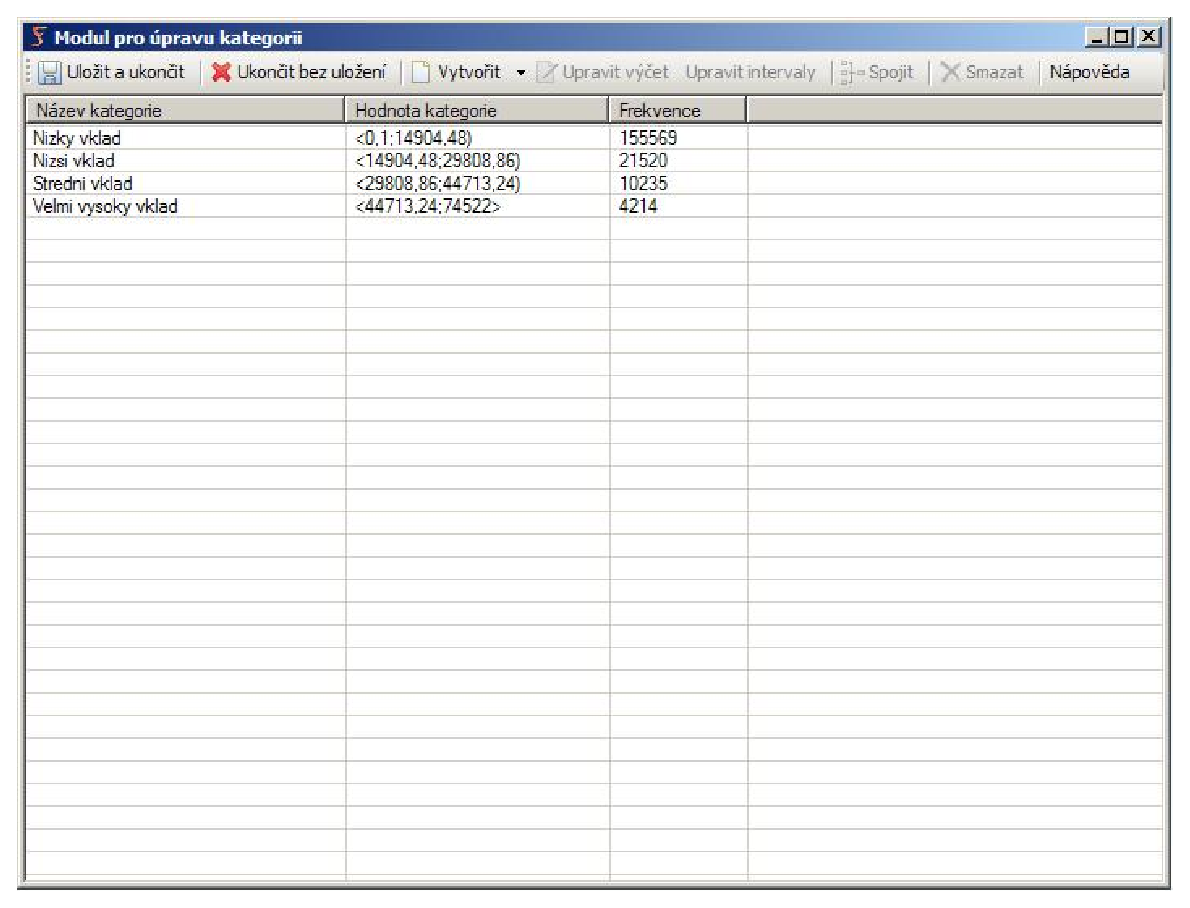
\includegraphics[width=14cm]{pics/editcategories_main.eps}
\caption{�prava kategori� -- hlavn� obrazovka}
\label{fig:editcategoriesmain}
\end{center}
\end{figure}

Na obr�zku \ref{fig:editcategoriesmain} je zobrazen seznam existuj�c�ch kategori�. Kategorie m��e b�t p�ejmenov�na 
standardn�m postupem pro p�ejmenov�n� polo�ky v seznamu GUI MS Windows, tj. dvoj�m pomal�m
kliknut�m na jej� n�zev, p��padn� kliknut�m na n�zev a stisknut�m klavesy F2 a pot� zad�n�m nov�ho n�zvu -- ilustruje obr�zek \ref{fig:editcategoriesrename}.
Proto�e kategorie mus� m�t navz�jem r�zn� n�zvy, po zad�n� nespr�vn�ho (ji� existuj�c�ho n�zvu)
bude ozn�mena chyba a kategorie se nep�ejmenuje.
\begin{figure}[!h]
\begin{center}
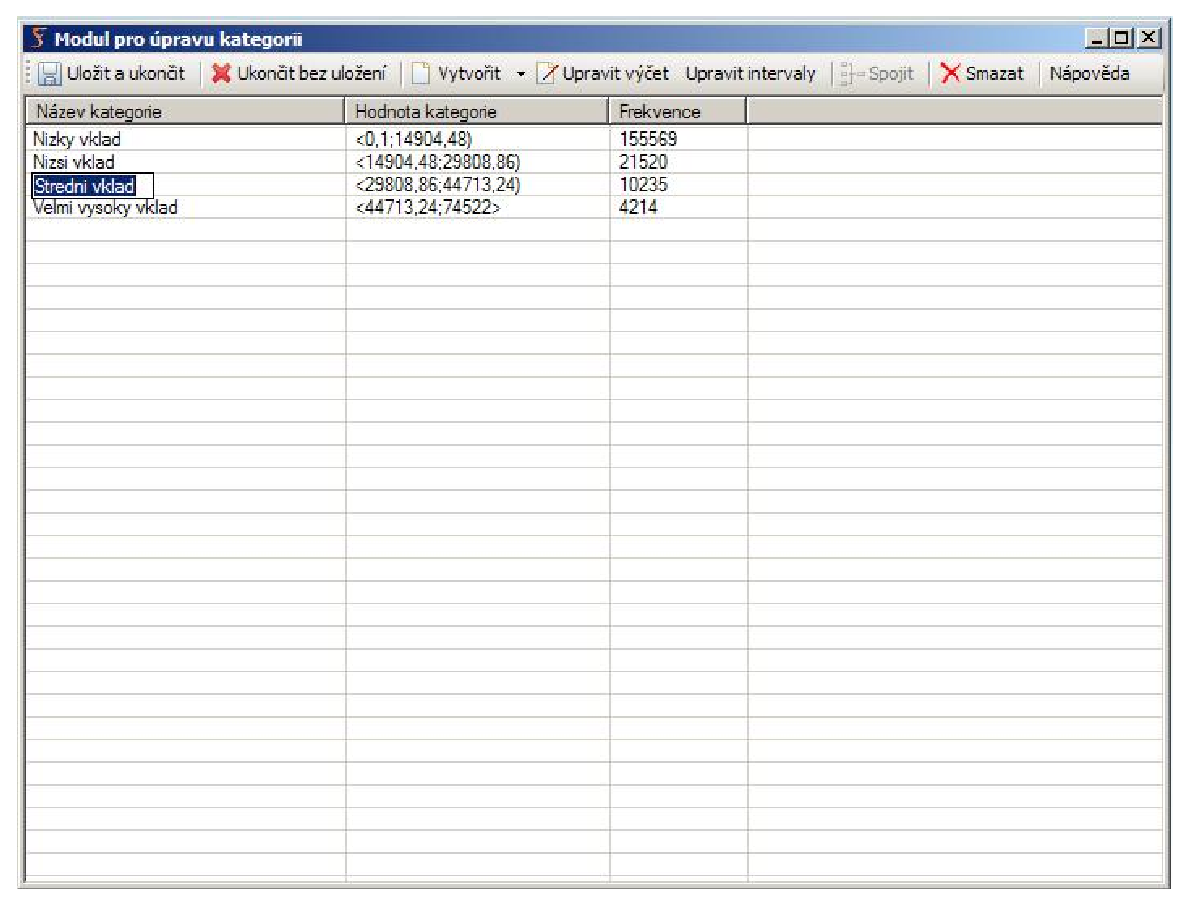
\includegraphics[width=14cm]{pics/editcategories_rename.eps}
\caption{�prava kategori� -- p�ejmenov�n� kategorie}
\label{fig:editcategoriesrename}
\end{center}
\end{figure}
\paragraph{}
V�ce kategori� m��e b�t spojeno do jedn� tak, �e s podr�en�m tla��tka Control p��padn� Shift
a kliknut�m na po�adovan� kategorie se vybere v�ce kategori� a pak kliknut�m na tla��tko ''Spojit''
se spoj� do jedn� kategorie.
\paragraph{}
Kategorie m��e b�t odstran�na z atributu vybran�m a n�sledn�m klik\-nu\-t�m na tla��tko ''Odstranit''.
\paragraph{}
Proveden� zm�ny v seznamu kategori� se ulo�� kliknut�m na tla��tko ''Ulo�it a zav��t''. Pokud
je pot�eba ukon�it pr�ci modulu bez ulo�en� zm�n, pou�ije se tla��tko ''Zav��t bez ulo�en�''.
U�ivatel m��e p�idat novou kategori� do seznamu kategori� v atributu. Z definice kategorie v metod� GUHA
a jej� n�sledn�ho roz���en� T.Kucha�em v \cite{kuchar} plyne, �e kategorie m��e obsahovat
intervaly a v��et hodnot.
\subsubsection{Obrazovka pro p�id�n� a �pravu interval�}
\begin{figure}[!h]
\begin{center}
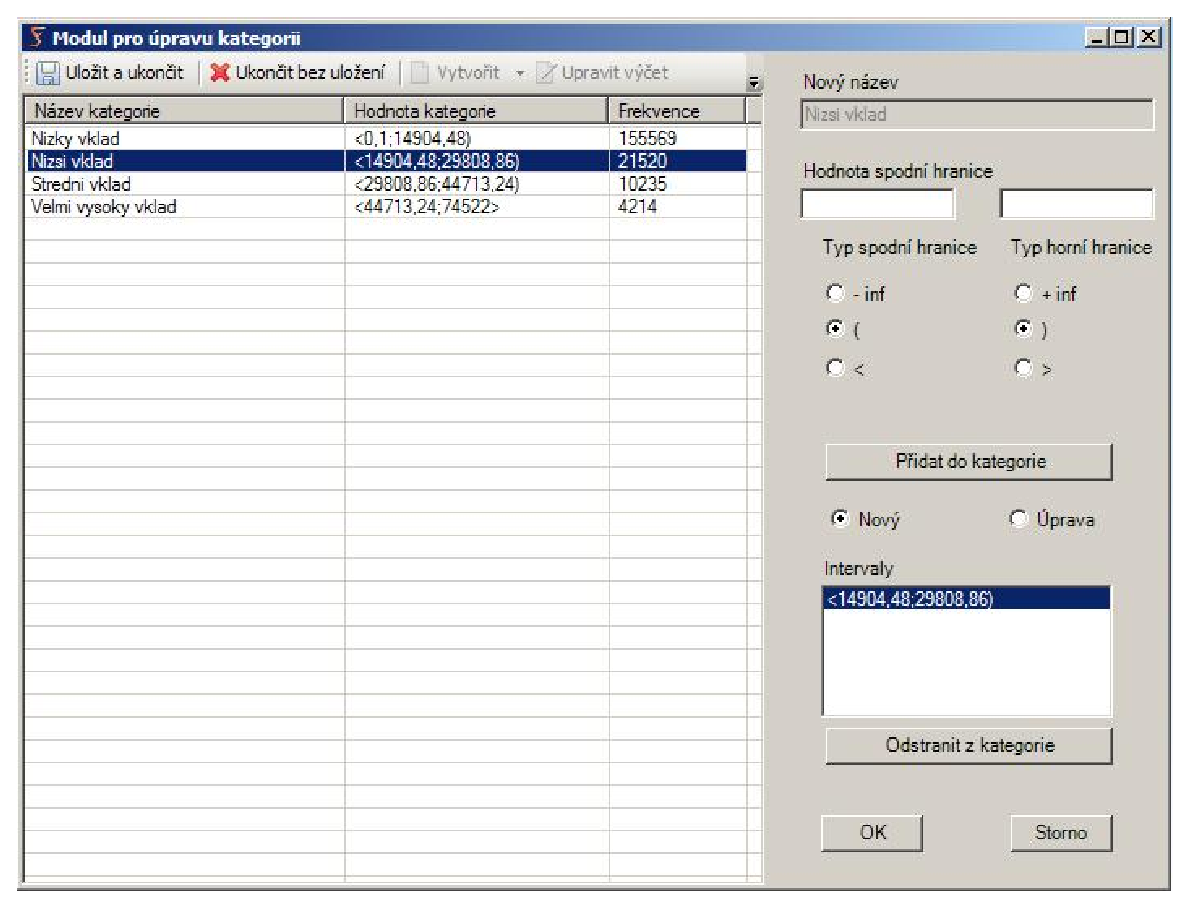
\includegraphics[width=14cm]{pics/editcategories_intervals.eps}
\caption{�prava kategori� -- pr�ce s intervaly}
\label{fig:editcategoriesintervals}
\end{center}
\end{figure}
Ve formul��i pro p�id�n� interval� (na obr�zku \ref{fig:editcategoriesintervals}) u�ivatel m��e p�id�vat intervaly
do nov� vytvo�en� kategorie. Ve formul��i lze vybrat typy hranic intervalu a hodnoty krajn�ch bod�,
pot� kliknut�m na tla��tko ''P�idat do kategorie'' p�idat interval do kategorie. Tento se pot� zobraz�
v seznamu interval� dan� kategorie a m��e b�t odebr�n zvolen�m a n�sledn�m kliknut�m na tla��tko pro odebr�n� intervalu. D�le se vybran� interval m��e upravovat p�epnut�m do re�imu �pravy.
\paragraph{}
P�i p�id�v�n� nebo zm�n� se kontroluje validita kategorie v atributu. Pro p�id�van� interval to tedy znamen�,
�e se zkontroluje jeho disjunktnost se st�vaj�c�mi intervaly v kategori�ch a tak� s hodnotami ve
v��tech kategori�. Pokud by p�id�van� interval nebyl disjunktn� s prvky existuj�c�ch kategori�,
modul ozn�m� chybu a nedovol� takov� interval do kategorie p�idat.
\paragraph{}
Po p�id�n� interval� do nov� vytv��en� kategorie lze potvrdit p�id�n� kategorie tla��tkem ''OK''.
Pro zru�en� p�id�n� kategorie se pou�ije tla��tko ''Storno''.
\paragraph{}
Obrazovka pro �pravu interval� v ji� existuj�c� kategorii se li�� t�m, �e nelze zm�nit n�zev kategorie
(ten lze zm�nit v hlavn� obrazovce). Logika p�i �prav� interval� v kategorii je stejn� jako je pops�no v��e.
\subsubsection{Obrazovka pro p�id�n� a �pravu v��tu}
\begin{figure}[!h]
\begin{center}
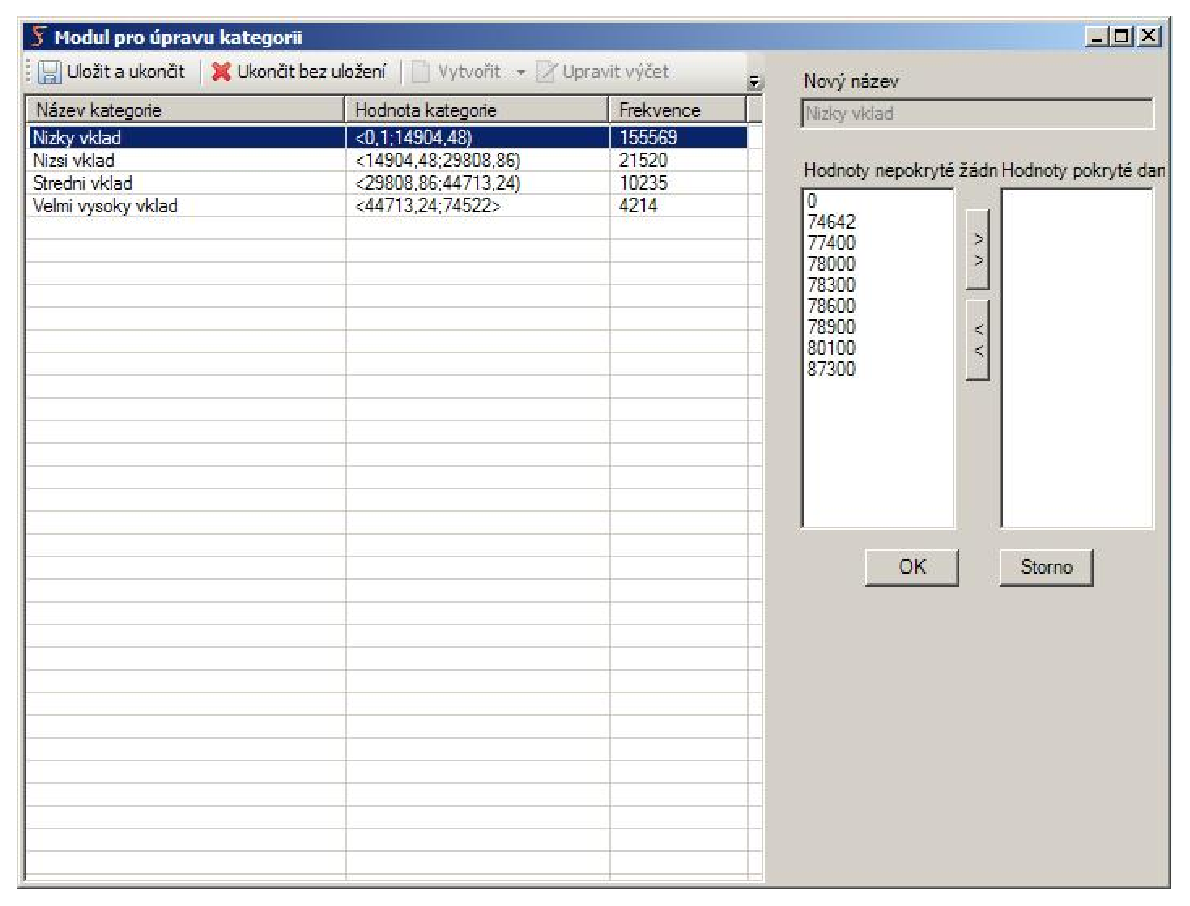
\includegraphics[width=14cm]{pics/editcategories_enum.eps}
\caption{�prava kategori� -- pr�ce s v��tem}
\label{fig:editcategoriesenums}
\end{center}
\end{figure}
Ve formul��i pro p�id�n� v��tu (na obr�zku \ref{fig:editcategoriesenums}) u�ivatel m��e p�id�vat hodnoty do v��tu
nov� vyt\-vo\-�en� kate\-gorie. Ve formul��i lze vybrat zat�m nepokryt� hodnoty v odpov�daj�c�m sloupci
a p�idat je do v��tu nov� vyt\-v��e\-n� kate\-gorie kliknut�m na p��slu�n� tla��tko. Hodnota
se pot� objev� ve v��tu hodnot dan� kategorie. Odtud m��e b�t odstran�na zvol�n�m a kliknut�m na
tla��tko pro odebr�n� hodnoty z v��tu.
Po p�id�n� hodnot do v��tu nov� vytv��en� kategorie lze potvrdit p�id�n� kategorie tla��tkem ''OK''.
Pro zru�en� p�id�n� kategorie se pou�ije tla��tko ''Storno''.
\chapter{Testy}
\label{tests}
V t�to kapitole bude prozkoum�n vliv r�zn�ch faktor� na b�h
�lohy s pou�it�m rela�n�ho roz���en� dataminingov� procedury.
Autor bude zkoumat vliv zejm�na velikosti dat a po�tu vygenerovan�ch
virtu�ln�ch sloupc�. Tak� se uk�e, �e pou�it�
bufferu pro bitov� �et�zky vygenerovan� virtu�ln�m atributem je z hlediska
v�konu nezbytn�.

\section[Zkouman� data]{Zkouman� datov� matice}
Zkouman� data vych�z� z datab�ze fiktivn� banky ''Barbora'' pou��van�
p�vodn� v projektu LISp-Miner a d�le Ferda DataMiner. Datab�ze obsahuje
data o fiktivn�ch klientech, jejich pohlav�, m�sta bydli�t�, transakc�ch, p�j�k�ch atd.
\subsection[Hlavn� matice]{Hlavn� datov� matice}
Hlavn� datov� matice s n�zvem ''Client\_Loans'' obsahuje �daje o jednotliv�ch klientech.
N�sleduj�c� tabulka obsahuje popis sloupc� hlavn� datov� matice.

\begin{table}[!h]
\begin{center}
\begin{tabular}{|l|l|l|}
\hline
N�zev sloupce & Typ sloupce & Popis sloupce \\
\hline
client\_id & Dlouh� cel� ��slo & Identifik�tor klienta  \\
\hline
loan\_id & Dlouh� cel� ��slo & Identifik�tor p�j�ky klienta  \\
															&&	(modelov�na situace, \\
															&&	 kde ka�d� klient m� jednu p�j�ku)\\
\hline
account\_id & Dlouh� cel� ��slo & Identifik�tor ��tu klienta  \\
															&&	(modelov�na situace, \\
															&&   kde ka�d� klient m� jeden ��et)\\
\hline
date & Dlouh� cel� ��slo & Datum zalo�en� ��tu  \\
\hline
amount & Dlouh� cel� ��slo & Velikost p�j�ky  \\
\hline
duration & Dlouh� cel� ��slo & Doba p�j�ky  \\
\hline
payments & Dlouh� cel� ��slo & V��e spl�tky  \\
\hline
status & text & Kvalita dluhu (subjektivn� hodnocen�)  \\
\hline
birth\_number & Dlouh� cel� ��slo & Rodn� ��slo  \\
\hline
DistrictID & Dlouh� cel� ��slo & Identifik�tor bydli�t�  \\
\hline
District & text & Bydli�t� \\
\hline
Region & text & Region \\
\hline
Inhabitants & Dlouh� cel� ��slo & Po�et obyvatel  \\
\hline
Muni499 & Dlouh� cel� ��slo & Po�et obc� v region�  \\
														&& s maxim�ln� 499 obyvateli \\
\hline
Muni1999 & Dlouh� cel� ��slo & Po�et obc� v region�  \\
														&& s maxim�ln� 1999 obyvateli \\
\hline
Muni9999 & Dlouh� cel� ��slo & Po�et obc� v region�  \\
														&& s maxim�ln� 9999 obyvateli \\
\hline
MuniOver & Dlouh� cel� ��slo & Po�et obc� v region�  \\
														&& s v�ce ne� 9999 obyvateli \\

\hline
Cities & Dlouh� cel� ��slo & Po�et m�st v regionu \\
\hline
PopulationRation & Dlouh� cel� ��slo &??\\
\hline
Salary & Dlouh� cel� ��slo & Pr�m�rn� plat v regionu\\
\hline
Unemployment95 & Dlouh� cel� ��slo & Nezam�stnanost v regionu v roce 1995\\
\hline
Unemployment96 & Dlouh� cel� ��slo & Nezam�stnanost v regionu v roce 1996\\
\hline
EnterpreneursRation & Dlouh� cel� ��slo & Podnikatel� v regionu \\
\hline
Crimes95 & Dlouh� cel� ��slo & Kriminalita v regionu v roce 1995\\
\hline
Crimes96 & Dlouh� cel� ��slo & Kriminalita v regionu v roce 1996\\
\hline
\end{tabular}
\end{center}
\caption{Sloupce hlavn� datov� matice ''Client\_Loans''}
\end{table}
\clearpage



\subsection[Vedlej�� matice]{Vedlej�� datov� matice}
Vedlej�� datov� matice ''trans\_pro\_client\_loan'' obsahuje transakce pro klienty
z tabulky ''Client\_Loans''. Pro ��ely testov�n� je tato tabulka obsa�ena
v datab�z� ve t�ech verz�ch: mal�, st�edn� a velk�, kde po�et ��dk� 
pro jednotliv� verze je
p�ibli�n� 10000, 70000 a 200000.
\paragraph{}
N�sleduj�c� tabulka obsahuje popis sloupc� vedlej�� datov� matice.

\begin{table}[!h]
\begin{center}
\begin{tabular}{|l|l|l|}
\hline
N�zev sloupce & Typ sloupce & Popis sloupce \\
\hline
trans\_id & Dlouh� cel� ��slo & Identifik�tor transakce  \\
\hline
client\_id & Dlouh� cel� ��slo & Identifik�tor klienta  \\
\hline
account\_id & Dlouh� cel� ��slo & Identifik�tor ��tu  \\
\hline
date & Dlouh� cel� ��slo & Datum transakce  \\
\hline
type & text & Typ transakce (p��jem, v�dej nebo v�b�r)  \\
\hline
operation & text & Typ operace (p�evod z / na ��et, v�b�r,  \\
&&vklad nebo v�b�r kartou)  \\
\hline
Amount & Dlouh� cel� ��slo & Velikost transakce  \\
\hline
Balance & Dlouh� cel� ��slo & Z�statek ??  \\
\hline
k\_symbol & Dlouh� cel� ��slo & Konstatn� symbol (��el transakce, nap�. inkaso)  \\
\hline
bank & text & Zdrojov� nebo c�lov� banka transakce  \\
\hline
account & Dlouh� cel� ��slo & Zdrojov� nebo c�lov� ��et transakce  \\
\hline
\end{tabular}
\end{center}
\caption{Sloupce vedlej�� datov� matice ''trans\_pro\_client\_loan''}
\end{table}

\section[�loha]{V�chodiska zad�n� a zadan� �loha}
Z�kladn� inspirac� pro �lohu pro rela�n� 4FT a SD4FT bylo zjistit n�jak� �daje
o objektech z hlavn� datov� matice na z�klad� �daj� z vedlej�� datov� matice.
V na�em p��pad� hled�me n�jak� vztahy v matici klient� na z�klad� �daj�
jak v hlavn� matici klient�, tak i ve vedlej�� matici jejich transakc�.
Pro SD4FT zkoum�me rozd�ly mezi dv�ma mno�inami.
\paragraph{}
Na z�klad� �daj� obsa�en�ch ve zkouman�ch datov�ch matic�ch a po diskuzi
s vedouc�m pr�ce bylo rozhodnuto za��t od jednodu���ch �loh pro
rela�n� proceduru a zapojovat je do �lohy pro b�n� 4ft Miner. V �loh�ch se zkoum�
status �v�ru v z�vislosti na r�zn�ch parametrech.

\subsection[4FT atribut]{4FT virtu�ln� boolsk� atribut}
\subsubsection[�loha 1]{�loha 1}
�loha je zadan� pro 4ft miner n�sleduj�c�m zp�sobem:

\begin{equation*}
District \& Salary \& \emph{TypeImplAmount} \Rightarrow_{90\%} LoanStatus
\end{equation*}

$\Rightarrow_{90\%}$ je v tomto p��pad� kvantifik�tor fundovan� implikace $Founded implication$
a \emph{TypeImplAmount} je virtu�ln� 4ft atribut s n�sleduj�c�m zad�n�m:

\begin{equation*}
Type \Rightarrow_{?} Amount
\end{equation*}

$\Rightarrow$ je v tomto p��pad� rovn� kvantifik�tor
fundovan� implikace $Founded implication$.


\subsection[V�sledky test�]{V�sledky test�}
V n�sleduj�c�ch tabulk�ch jsou uvedeny doby b�hu �loh
s r�zn�mi velikostmi vedlej�� datov� matice a po�tem relevantn�ch
ot�zek vygenerovan�ch rela�n�m 4ft booleovsk�m atributem.
\paragraph{}
Ka�d� test se pou�t�l t�ikr�t a v�sledn� �as se zpr�m�roval. Mezi ka�d�m spu�t�n�m
Ferda DataMiner byl znovu spu�t�n, aby byly zachov�ny stejn� podm�nky pro jednotliv�
b�hy (bez tohoto by se p�i druh�m a dal��m spu�t�n� na��taly informace pro krabi�ky z cache).
\subsubsection{�loha 1}
\begin{table}[!h]
\begin{center}
\begin{tabular}{|l|l|l|l|}
\hline
Transakce / & mal� & st�edn� &  velk�  \\
\# rel.otazek&&&\\
\hline
16 & 14s & 25s & 1m 10s\\
\hline
50 & 15s & 25s & 1m 32s \\
\hline
80 & 9m 2s & 11m 11s& 12m 2s\\
\hline
100 & 12m & 24m & 1h 3m \\
\hline
\end{tabular}
\end{center}
\caption{Test rela�n�ho 4ft mineru: �loha 1}
\end{table}

\subsubsection{�loha 1 -- bez cache}
Zde byla zkoum�na rychlost pr�ce bez cache. Porovn�n�m s p�edchoz� tabulkou lze zjistit
�asov� rozd�ly b�hu �lohy.
\begin{table}[!h]
\begin{center}
\begin{tabular}{|l|l|l|l|}
\hline
Transakce / & mal� & st�edn� &  velk�   \\
\# rel.otazek&&&\\
\hline
16 & 21s & 1m8s & 6m 45s\\
\hline
50 & 45s & 3m 5s & 26m 33s \\
\hline
100 & 50m 30s & 9h 52m& --\footnotemark  \\
\hline
\end{tabular}
\end{center}
\caption{Test rela�n�ho 4ft mineru: �loha 1 -- bez cache}
\end{table}
\paragraph{}
\paragraph{}
\subsection[SD4FT atribut]{SD4FT virtu�ln� boolsk� atribut}
\subsubsection[�loha]{V�chodiska zad�n� a zadan� �loha}
�loha je zadan� pro 4ft miner n�sleduj�c�m zp�sobem:

\begin{equation*}
District \& Salary \& \emph{TypeImplAmountBank} \Rightarrow_{90\%} LoanStatus
\end{equation*}

$\Rightarrow_{90\%}$ je v tomto p��pad� kvantifik�tor fundovan� implikace $Founded implication$
a \emph{TypeImplAmountBank} je virtu�ln� SD4ft atribut s n�sleduj�c�m zad�n�m:

\begin{equation*}
Type \Rightarrow_{?} Amount (Bank)
\end{equation*}

$\Rightarrow$ je v tomto p��pad� rovn� kvantifik�tor
fundovan� implikace $Founded implication$.
\subsection[V�sledky test�]{V�sledky test�}
V n�sleduj�c�ch tabulk�ch jsou uvedeny doby b�hu �loh
s r�zn�mi velikostmi vedlej�� datov� matice a po�tem relevantn�ch
ot�zek vygenerovan�ch rela�n�m SD4ft booleovsk�m atributem.
\subsubsection{�loha 1}
\begin{table}[!h]
\begin{center}
\begin{tabular}{|l|l|l|l|}
\hline
Transakce / & mal� & st�edn� &  velk� \\
\# rel.otazek&&&\\
\hline
16 &8m01s&13m05s&21m30s\\
\hline
40 &16m12s&28m57s&29m30s\\
\hline
80 &25m40s&35m20s&58m05s\\
\hline
100 &30m34s&55m50s&1h13m50s\\
\hline
\end{tabular}
\end{center}
\caption{Test rela�n�ho SD4ft mineru: �loha 1}
\end{table}
\footnotetext{Vzhledem k velmi dlouh� p�edpokl�dan� dob� b�hu
test nebyl spou�t�n}
\section{Z�v�r}
Z proveden�ch test� plyne, �e doba b�hu pro ob� �lohy z�le�� hlavn�
na po�tu vygenerovan�ch virtu�ln�ch sloupc�. Velikost vedlej�� datov� matice
sice m� na �lohu vliv, rozhoduj�c�m faktorem v�ak z�st�v� pr�v� po�et vygenerovan�ch
sloupc�. To vypl�v� ze zp�sobu,
jak�m virtu�ln� atribut funguje: p�i prvn�m generov�n� spo��t� bitov� �et�zky
a ulo�� si je do bufferu, p�i dal��ch vol�n�ch se pracuje s bufferem. Proto
p�i r�zn�ch velikostech vedlej�� datov� matice se �m�rn� m�n� pouze
doba prvn�ho generov�n�.
\paragraph{}
D�le se n�zorn� ukazuje pot�eba bufferu pro bitov� �et�zky generovan�
virtu�ln�m atributem. Lze to zjistit jak z �as� v tabulce,
tak i z faktu, �e p�i testov�n� s vypnutou cache byl testovac�
po��ta� p�i b�hu �lohy vyt�en o pozn�n� v�ce.
\paragraph{}
Tak� je pot�eba uv�st, �e implementace rela�n�ch roz���en� v r�mci dan� pr�ce
je pilotn� a chov�n� �loh s hypot�zov�m virtu�ln�m atributem vy�aduje dal��
zkou�en� a zkoum�n�, stejn� jako tomu bylo v p��pad� j� implementovan�ch
dataminingov�ch �loh.
\chapter{Zhodnocen� pr�ce}
\label{conclusion}
\section{Spln�n� c�l�}
\paragraph{}
V t�to kapitole prob�hne shrnut� v�sledk� dan� diplomov� pr�ce.
\subsection{Pilotn� implementace}
\paragraph{}
Implementace rela�n�ch roz\-��\-�e\-n� data\-miningov�ch pro\-ce\-dur by\-la
zce\-la no\-v�m �kolem pro pro\-st�ed� Ferda Data\-Miner. P�ed\-t�m
tato roz\-���en� ne\-byla realizov�na ani v prvn� verzi
pro\-st�ed� Ferda Data\-Miner, ani v r�mci sys\-t�mu LISp-Miner (a�\-koliv
exis\-tovala n�jak� pi\-lotn� implementace, se kterou autor nep�i�el do styku
a od jej�ho rozvoje a u��van� se upustilo).
\paragraph{}
Teoretick� p��prava pro implementaci rela�n�ch roz���en� byla vykon�na T.Karbanem
ve sv� dizerta�n� pr�ci \uv{DATA MINING
IN RELATIONAL DATABASES} uveden� v seznamu pou�it� literatury jako \cite{relminer}.
A�koliv tato pr�ce je rovn� implementa�n�, k okam�iku zah�jen� i dokon�en� dan� diplomov�
pr�ce dle informac� p��mo od vedouc�ho dizerta�n� pr�ce J.Raucha
nebyl k dispozici funk�n� spustiteln� program. Proto implementaci v dan� diplomov� pr�ci
lze br�t jako pilotn�, v �em� spo��v� jak jej� p��nos, tak i zji�t�n� omezen� ji� zm�n�na
v tomto textu.
\subsection{Spln�n� c�le ze zad�n�}
\paragraph{}
Jak ji� bylo zm�n�no, byly implementov�ny rela�n� roz���en�
st�vaj�c�ch dataminingov�ch procedur 4FT a SD4FT. Odpov�daj�c� krabi�ky
v prost�ed� Ferda se jmenuj� \uv{Virtu�ln� booleovsk� 4FT atribut} a
\uv{Virtu�ln� booleovsk� SD4FT atribut}. Implementuj� hypot�zov�
virtu�ln� atribut, kter� je rela�n�m roz���en�m pro procedury 4FT a SD4FT
a t�m tedy p��mo spl�uj� zad�n� pr�ce. 
\paragraph{}
D�le byl implementov�n agrega�n� virtu�ln� atribut. Odpov�daj�c� krabi�ka v prost�ed� Ferda
se jmenuje \uv{Agrega�n� virtu�ln� sloupec}. T�mto se spl�uje zad�n� pr�ce, proto�e pat�� do rela�n�ch roz���en�
dataminingov�ch procedur.
\paragraph{}
Tak� byly implementov�ny krabi�ky pro transformaci atribut� pro vyt\-vo\-�e\-n� ekvi\-distan�\-n�ch 
interval�,
ekvi\-frekven�\-n�ch interval� a krabi�ka pro p��\-mou �p\-ra\-vu at\-ri\-bu\-tu. Tyto �lohy
p�vodn� nepat�ily do zad�n�, av�ak v odevzdan� diplomov� pr�ci Tom�e Kucha�e
\cite{kuchar} nebyly rovn� z r�zn�ch d�vod� p��tomny a
uk�zalo se, �e by bylo velmi ��douc� je m�t implementovan� co nejd��ve. Umo��uj�
podstatn� roz���en� zp�sob� zad�van� data\-miningov�ch �loh a t�mto v�razn�
p�isp�ly k lep��m v�sledk�m i t�to diplomov� pr�ce. Zad�n� pr�ce bylo roz���eno o po�adavek
implementace t�chto metod, kter� byl spln�n. Jedn� se tedy o napln�n� c�l� pr�ce.
\subsection{P��prava pro budouc� implementace}
\paragraph{}
V pr�b�hu pr�ce byly navr�eny takov� 
zm�ny st�vaj�c�ch jednotliv�ch prvk� syst�mu Ferda DataMiner, aby rela�n�
roz���en� mohla b�t relativn� snadno implementov�na i pro jin� dataminingov�
procedury, ne� pro ty, kter� implementoval autor t�to pr�ce. Jin�mi slovy,
c�lem a p��nosem dan� diplomov� pr�ce byla i p��prava prost�ed� Ferda
DataMiner pro snadn�j�� dal�� v�voj. Autor pr�ce tedy tvrd�, �e tento c�l, kter�
 (by� ne explicitn�) vych�z� ze zad�n�, byl v dan� diplomov� pr�ci spln�n.
\section{Doporu�en� dal��ho sm�ru pr�ce}
\paragraph{}
V t�to kapitole bude nazna�en mo�n� sm�r dal��ho v�voje rela�n�ch roz���en� pro
dataminingov� procedury v prost�ed� Ferda DataMiner.
\subsection{Roz���en� pro zb�vaj�c� procedury}
\paragraph{}
Jak j� bylo zm�n�no, lze pom�rn� snadno implementovat rela�n� roz���en�
pro zb�vaj�c� dataminingov� procedury z prost�ed� Ferda DataMiner. K okam\-�i\-ku
odevzd�n� diplomov� pr�ce je v prost�ed� implementov�no 6 (nerela�n�ch) procedur, lze
tedy d�le uva�ovat o rela�n�ch roz���en�ch pro KL a SDKL, d�le pro CF a SDCF.
Tyto autorem nebyly implementov�ny z d�vod� toho, �e c�lem pr�ce bylo krom� samotn�ho naprogramov�n� tak�
vytvo�en� z�kladu pro rela�n� roz���en� v prost�ed� Ferda DataMiner, vy�e�it obecn�
probl�my, kter� p�i implementaci vznikly a otestovat chov�n� vytvo�en�ch
roz���en�. Nav�c zp�sob implementace je stejn� jako pro j� vytvo�en�
roz���en�, nejednalo by se tedy o podstatn� p��nos k pr�ci.
\subsection{Re�ln� hypot�zov� atribut}
\paragraph{}
Logick�m sm�rem dal��ho roz�i�ov�n� se jev� implementace
obecn�j��ho hypot�zov�ho atributu, kter� produkuje virtu�ln� sloupce
skl�daj�c� se z re�l\-n�ch ��sel (a ne pouze z hodnot \emph{true} a \emph{false}).
Takov� atribut m��e d�vat na v�stup tyto sloupce bu� rovnou jako fuzzy
bitov� �et�zce anebo je bude p�ed�vat dal��m modul�m ke zpracov�n�. Fuzzy bitov�
�et�zce sice zat�m nejsou v prost�ed� Ferda DataMiner implementov�ny,
av�ak dle T.Kuchare (\cite{kuchar}) syst�m generov�n� m��e b�t o n� roz���en.
Tot� plat� i pro rela�n� roz���en� -- syst�m generov�n� virtu�ln�ch sloupc�
m��e b�t pom�rn� snadno upraven pro sloupce re�ln�ch ��sel.
\subsection{Nov� modul pro prohl�en� v�sledk�}
\paragraph{}
Pro lep�� pr�ci s hypot�zami generovan�mi z �loh, kter� pou��vaj�
nov� vytvo�en� rela�n� roz���en� procedur, je nutn� roz���it
mo�nosti sou�asn�ho modulu pro prohl�en� v�sledk�. Ten zobrazuje atributy v hypot�z�ch
ve form� prost�ho textu, co� dosta�uje pro prohl�en� v�sledk� s pou�it�m
ne\-re\-la�\-n�ch atribut�, av�ak pro rela�n� atributy by bylo vhodn� m�t mo�nost pracovat s atributy ze zad�n�
pod�lohy zvl᚝  -- te� se zobraz� vcelku jako jeden textov� �et�zec.
\section{Z�v�r}
\paragraph{}
Na z�klad� v��e uveden�ho autor prohla�uje c�le sv� diplomov� pr�ce za spln�n�.
\thebibliography{bo}
\bibitem{guhabasic} H�jek, P. � Havr�nek, T.:
Mecha\-nizing Hypo\-thesis Formation � Mathematical
Foundations for a General Theory. 
Springer-Verlag, 1978, ISBN: 3-540-08738-9,
available for download at 
http://www.cs.cas.cz/~hajek/guhabook/
\bibitem{guha} Rauch J., �im�nek M.: 
GUHA Method and Granular Computing. In: Hu X., Liu Q.,
Skowron A., Lin T. Y., Yager R., Zang B. (ed.). 
Proceedings of IEEE konference Granular Computing 2005.
2005, s. 630�635.
\bibitem{relminer} Karban, T.: Prvn� praktick� zku�enosti
s Rel\-Minerem, viz
http://146.102.64.29/%7Esvatek/keg/seminar/keg-sem.html
\bibitem{mlrules} Rauch J.: RAUCH, Jan. Interesting
Association Rules
and Multi\-relational Association Rules.
Taiwan 06.05.2002. In: LEE, H. C., LAI, F. (ed.).
Communications of IICM. Taipei : IICM, 2002, s. 77�82
\bibitem{altrules} Rauch J., �im�nek M.: 
An Alternative Approach to Mining Association Rules.
In: Lin, T. Y. � Ohsuga, S. � Liau, C. J. � Hu, X. � Tsumot,
S. (ed.): Foundations of Data Mining and Knowledge Discovery. 
Berlin: Springer, 2005, pp. 211 � 232
\bibitem{ferda} Kov�� M., Kucha� T., Kuzmin A., Ralbovsk� M.: 
Ferda, nov� vizu�ln� prost�ed� pro dob�v�n� znalost�.
P�ijato k prezentaci na konferenci ZNALOSTI 2006, 
viz http://fim.uhk.cz/znalosti/index.php?p=prispevky
\bibitem{duchacek} Duch��ek M.: N�stroj pro spr�vu datab�z�
s vyu�it�m pro multi\-rela�n� data\-mining,
diplomov� pr�ce na Kated�e softwarov�ho in�en�r\-stv�, 2006
\bibitem{kuchar} Kucha� T.:Experiment�ln� GUHA procedury,
diplomov� pr�ce na Kated�e softwarov�ho in�en�r\-stv�, 2006
\bibitem{apriori} Aggraval, R. et al.: Fast Discovery 
of Association Rules. In Fayyad, U.M. et al.: Advances 
in Knowledge Discovery and Data Mining, 
pp. 307-328, AAAI Press / MIT Press, 1996

\listoftables
\listoffigures

\appendix
\chapter{Zdrojov� k�dy}
\section[Seznam soubor�]{Seznam zm�n�n�ch a vytvo�en�ch soubor�}
Jako sou��st dan� diplomov� pr�ce byly vytvo�eny nebo upraveny
soubory se zdrojov�mi k�dy. Na projektu Ferda DataMiner pracuje
v sou�asn� dob� v�ce lid�. Zdrojov� k�dy jsou proto spravov�ny
syst�mem Subversion a nach�zej� se
na \verb+https://svn.sourceforge.net/svnroot/ferda+.  K diplomov� pr�ci autora
se vztahuj� zm�ny proveden� autorem \emph{kuzmos} od ��sla revize 292.

\paragraph{}
\begin{itemize}
\item \verb+ferda/slice/Modules/Guha.MiningProcessor.ice+
\item \verb+ferda/slice/Modules/Boxes/DataPreparation/DataPreparation.ice+
\item \verb+ferda/slice/Modules/Common.ice+
\item \verb+ferda/src/FrontEnd/AddIns/ResultBrowser/+
\item \verb+ferda/src/FrontEnd/AddIns/EditCategories/+
\item \verb+ferda/src/Modules/BoxModulesServices/Boxes/+
\newline
\verb+*.xml+
\newline
Drobn� zm�ny pro pr�ci s nov�mi atributy.
\item \verb+ferda/src/Modules/BoxModulesServices/DataPreparation/+
\newline
\verb+Categorization/Common.cs+
\item \verb+ferda/src/Modules/BoxModulesServices/DataPreparation/+
\newline
\verb+Categorization/EachValueOneCategory/+
\newline
Drobn� zm�ny existuj�c�ho k�du pro pr�ci s virtu�ln�m agrega�n�m atributem.
\item \verb+ferda/src/Modules/BoxModulesServices/DataPreparation/+
\newline
\verb+Categorization/EquidistantIntervals+
\item \verb+ferda/src/Modules/BoxModulesServices/DataPreparation/+
\newline
\verb+Categorization/EquifrequencyIntervals+
\item \verb+ferda/src/Modules/BoxModulesServices/DataPreparation/+
\newline
\verb+Categorization/StaticAttribute+
\item \verb+ferda/src/Modules/BoxModulesServices/DataPreparation/+
\newline
\verb+DataSource/VirtualColumn+
\item \verb+ferda/src/Modules/BoxModulesServices/GuhaMining/+
\newline
\verb+VirtualAttributes/VirtualFFTBooleanAttribute+
\item \verb+ferda/src/Modules/BoxModulesServices/GuhaMining/+
\newline
\verb+VirtualAttributes/VirtualSDFFTBooleanAttribute+
\item \verb+ferda/src/Modules/Core/MiningProcessor/Miners/+
\newline
�pravy v souborech \verb+FourFoldMiningProcessor.cs+ a \verb+SDFourFoldMiningProcessor.cs+,
kde byly vytvo�eny samotn� procedury pro rela�n� mining. �pravy v souborech \verb+MinningProcessor.cs+ a \verb+MiningProcessorFunctionsI.cs+ pro zaji�t�n� funk�nosti pr�ve vytvo�en�ch a v budoucnu
vytv��en�ch rela�n�ch roz���en�.
\item \verb+ferda/src/Modules/Core/MiningProcessor/+
\newline
\verb+QuantifierEvaluator/FirstNNoResult.cs+
\item \verb+ferda/src/Modules/Core/MiningProcessor/+
\newline
\verb+Generation/LeafEntities.cs+
\newline
P�id�na procedura pro generov�n� bitov�ch �et�zk� pro rela�n� roz���en�.
\end{itemize}

\section[P�id�n� nov�ch rela�n�ch roz���en�]{Postup pro p�id�n� nov�ch rela�n�ch roz���en�}
\subsection[Krabi�ka]{Vytvo�en� krabi�ky}
Pro u�ivatelsk� rozhran� se mus� vytvo�it krabi�ka pro syst�m Ferda DataMiner. Obecn� n�vod
pro tento postup je pops�n v dokumentu ''Implementace krabi�ek'', kter� se nach�z� v repozit��i
zdrojov�ch k�du prost�ed� Ferda DataMiner jako \verb+ferda/docsrc/draft/implementaceKrabicek.xdb+.
Jako vzorovou krabi�ku pro implementaci rela�n�ch roz���en� se m��e pou��t jedna z krabi�ek
\verb+VirtualFFTBooleanAttribute+ nebo \verb+VirtualSDFFTBooleanAttribute+. Nesm� se zapomenout
na �pravu soubor� \newline \verb+ferda/src/Modules/BoxModulesServices/Boxes/*.xml+
\subsection[Backend]{�prava procedur v backendu}
Zde se v podstat� jedn� o implementaci procedury \verb+TraceBoolean+ vracej�c� enumer�tor
bitov�ch �et�zk� v jednotliv�ch procedur�ch, kter� se nach�zej� v
\verb+ferda/src/Modules/Core/MiningProcessor/Miners+. Jako vzor implementace m��e op�t
poslou�it doty�n� procedura implementov�na pro \newline \verb+FourFoldMiningProcessor.cs+ nebo
\verb+SDFourFoldMiningProcessor.cs+. Zb�vaj�c� �pravy pro zaji�t�n� funk�nosti rela�n�ch roz���en�
byly implementov�ny autorem dan� diplomov� pr�ce pro uleh�en� p�id�v�n� roz���en�
dal��ch procedur.

\chapter{Obsah p�ilo�en�ho CD}
\label{cdrom}
\paragraph{}
Na p�ilo�en�m CD se nach�z� aktu�ln� svn reposit�� pro projekt Ferda DataMiner.
Implementace v r�mci t�to diplomov� pr�ce je sou��st� projektu, pro �sp�nou kompilaci 
se tedy zdrojov� k�dy p�ikl�daj� v pln�m rozsahu. Podrobn� seznam zm�n�n�ch soubor� je sou��st�
dodatku \ref{sourcecode}. Text t�to pr�ce je rovn� sou��st� reposit��e a nach�z� se v adres��i
\verb+publications/diplomky/kuzmos/+. Pro pohodl� jsou v adres��i \verb+docs+ p�ilo�eny d�le�it� dokumenty
nap��klad pro instalaci,
jejich� zdrojov� k�dy se nach�zej� v reposit��i v \verb+ferda/docsrc/+. D�le je sou��st� CD
datab�ze fiktivn� banky Barbora, na kter� byly prov�d�ny testy z kapitoly \ref{tests}. Soubor se nach�z�
v adres��i \verb+data/+.
\end{document}
